\documentclass[a4paper,13pt]{extreport}
\usepackage{graphicx}
%\usepackage{indentfirst}
\usepackage{mathptmx}
\usepackage{amsmath,amsfonts,amssymb,fancyhdr}
\usepackage{amsthm,amsxtra,latexsym, amscd}
\usepackage{bm}
\usepackage[utf8]{vietnam}
%\usepackage[unicode,colorlinks=true]{hyperref} 
%\usepackage[utf8]{inputenc}
\usepackage[left=3.50cm, right=2.00cm, top=3.00cm, bottom=3.50cm]{geometry}
\usepackage{tocloft}
\usepackage{type1cm}
\usepackage{vector}
\usepackage{color}
\usepackage[usenames,dvipsnames]{xcolor}
\usepackage{caption/subcaption}
\usepackage[section]{placeins}
%\usepackage{subfigure}
\usepackage{pbox}
%\usepackage[unicode,colorlinks=true]{hyperref}
\usepackage{framed}

\usepackage[hyphens]{url}
%\usepackage[hidelinks]{hyperref}
\usepackage[ unicode, plainpages = false, pdfpagelabels, 
pdfpagelayout = OneColumn, % display single page, advancing flips the page - Sasa Tomic
bookmarks,
bookmarksopen = true,
bookmarksnumbered = true,
breaklinks = true,
linktocpage,
pagebackref,
colorlinks = true,
linkcolor = blue,
urlcolor  = blue,
citecolor = red,
anchorcolor = green,
hyperindex = true,
hyperfigures
]{hyperref} 


%\usepackage{algorithm2e}
\usepackage[chapter]{algorithm}
\usepackage{algpseudocode}
\usepackage{setspace}
\makeatletter
\newcommand{\newalgname}[1]{%
	\renewcommand{\ALG@name}{#1}%
}
\usepackage{longtable}
\usepackage[acronym]{glossaries}
\usepackage{multicol}
\setlength{\columnsep}{25pt}
\usepackage{nomencl}
\makenomenclature
\usepackage{multirow}
\usepackage{pdfpages}

\usepackage{tabularx}
\captionsetup{compatibility=false}
\renewcommand\cftchappresnum{\chaptername\space}
\setlength{\cftchapnumwidth}{2.5cm}
\usepackage{titlesec}
\titleformat{\chapter}[display]
{\normalfont\large\bfseries\centering}{\chaptertitlename\ \thechapter}{20pt}{\huge}
\linespread{1.3}

%\baselineskip 19.5 pt
                 

\begin{document}
	
	%
\includepdf[pages=1]{docs/BiaChinh}
	
\includepdf{docs/BiaPhu}
	%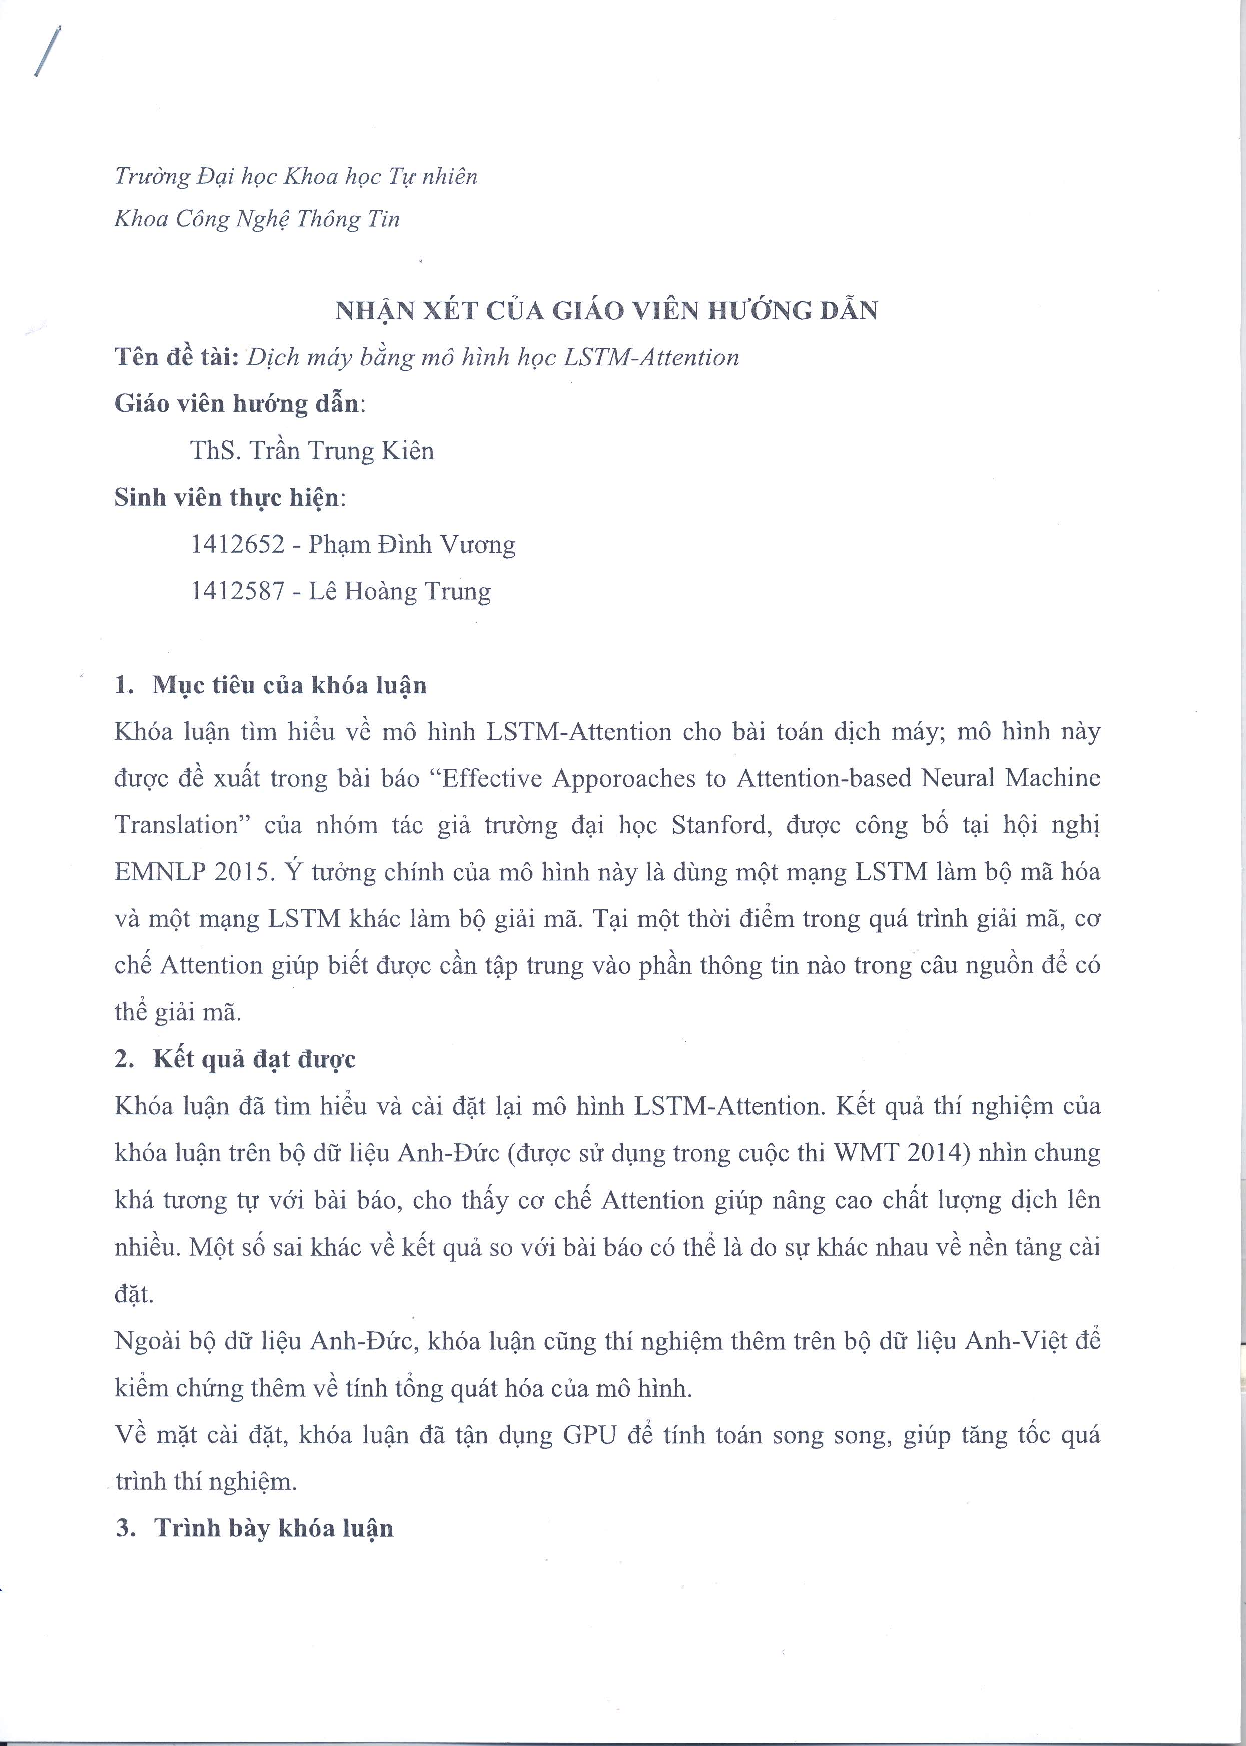
\includepdf[pages=1-2]{docs/NhanXet}
	
	\pagenumbering{roman}
	\newpage
\chapter*{LỜI CẢM ƠN}
\addcontentsline{toc}{chapter}{LỜI CẢM ƠN}
%\hspace{0.3in}
Lời đầu tiên, chúng em xin được gửi lời tri ân vô cùng sâu sắc đến thầy hướng dẫn khóa luận tốt nghiệp của chúng em - Thầy Trần Trung Kiên. Thầy đã rất tận tâm, nhiệt tình hướng dẫn và động viên chúng em trong suốt quá trình làm khóa luận. Nếu không có sự quan tâm, theo dõi chặt chẽ của Thầy chắc chắn chúng em không thể hoàn thành khóa luận này. Thầy còn giúp chúng em hình thành được một nền tảng rất vững chắc và củng cố lại những kiến thức trong suốt quãng đường Đại học.

Em xin chân thành cảm ơn quý Thầy Cô khoa Công nghệ Thông tin - trường Đại học Khoa học Tự nhiên - ĐHQG-HCM, những người đã ân cần giảng dạy cho chúng em những kiến thức vô cùng cần thiết, bổ ích để chúng em có thể vững bước trên con đường sau này.

Con xin cảm ơn ba mẹ đã sinh thành, nuôi dưỡng và dạy dỗ để chúng con có được thành quả như ngày hôm nay. Ba mẹ luôn là nguồn động viên, nguồn sức mạnh hết sức lớn lao mỗi khi chúng con gặp khó khăn trong cuộc sống. Có bố mẹ ủng hộ, chúng con luôn luôn cảm thấy an tâm để tiếp tục tiến lên phía trước.

Chúng em cũng xin gửi lời cảm ơn chân thành và sâu sắc tới anh Trần Duy Quang cùng với anh chị, bạn bè đồng nghiệp trong công ty AIOZ đã hỗ trợ, giúp đỡ chúng em về mặt phần cứng để có thể thuận lợi hoàn thành khóa luận này.



\hfill Tp.Hồ Chí Minh, 07/2018

\hfill \textit{Phạm Đình Vương}

\hfill \textit{Lê Hoàng Trung}

	
	%\newpage
	%\thispagestyle{empty}
	%\mbox{}
	
	%\newpage
	%\addcontentsline{toc}{chapter}{ĐỀ CƯƠNG CHI TIẾT}
	%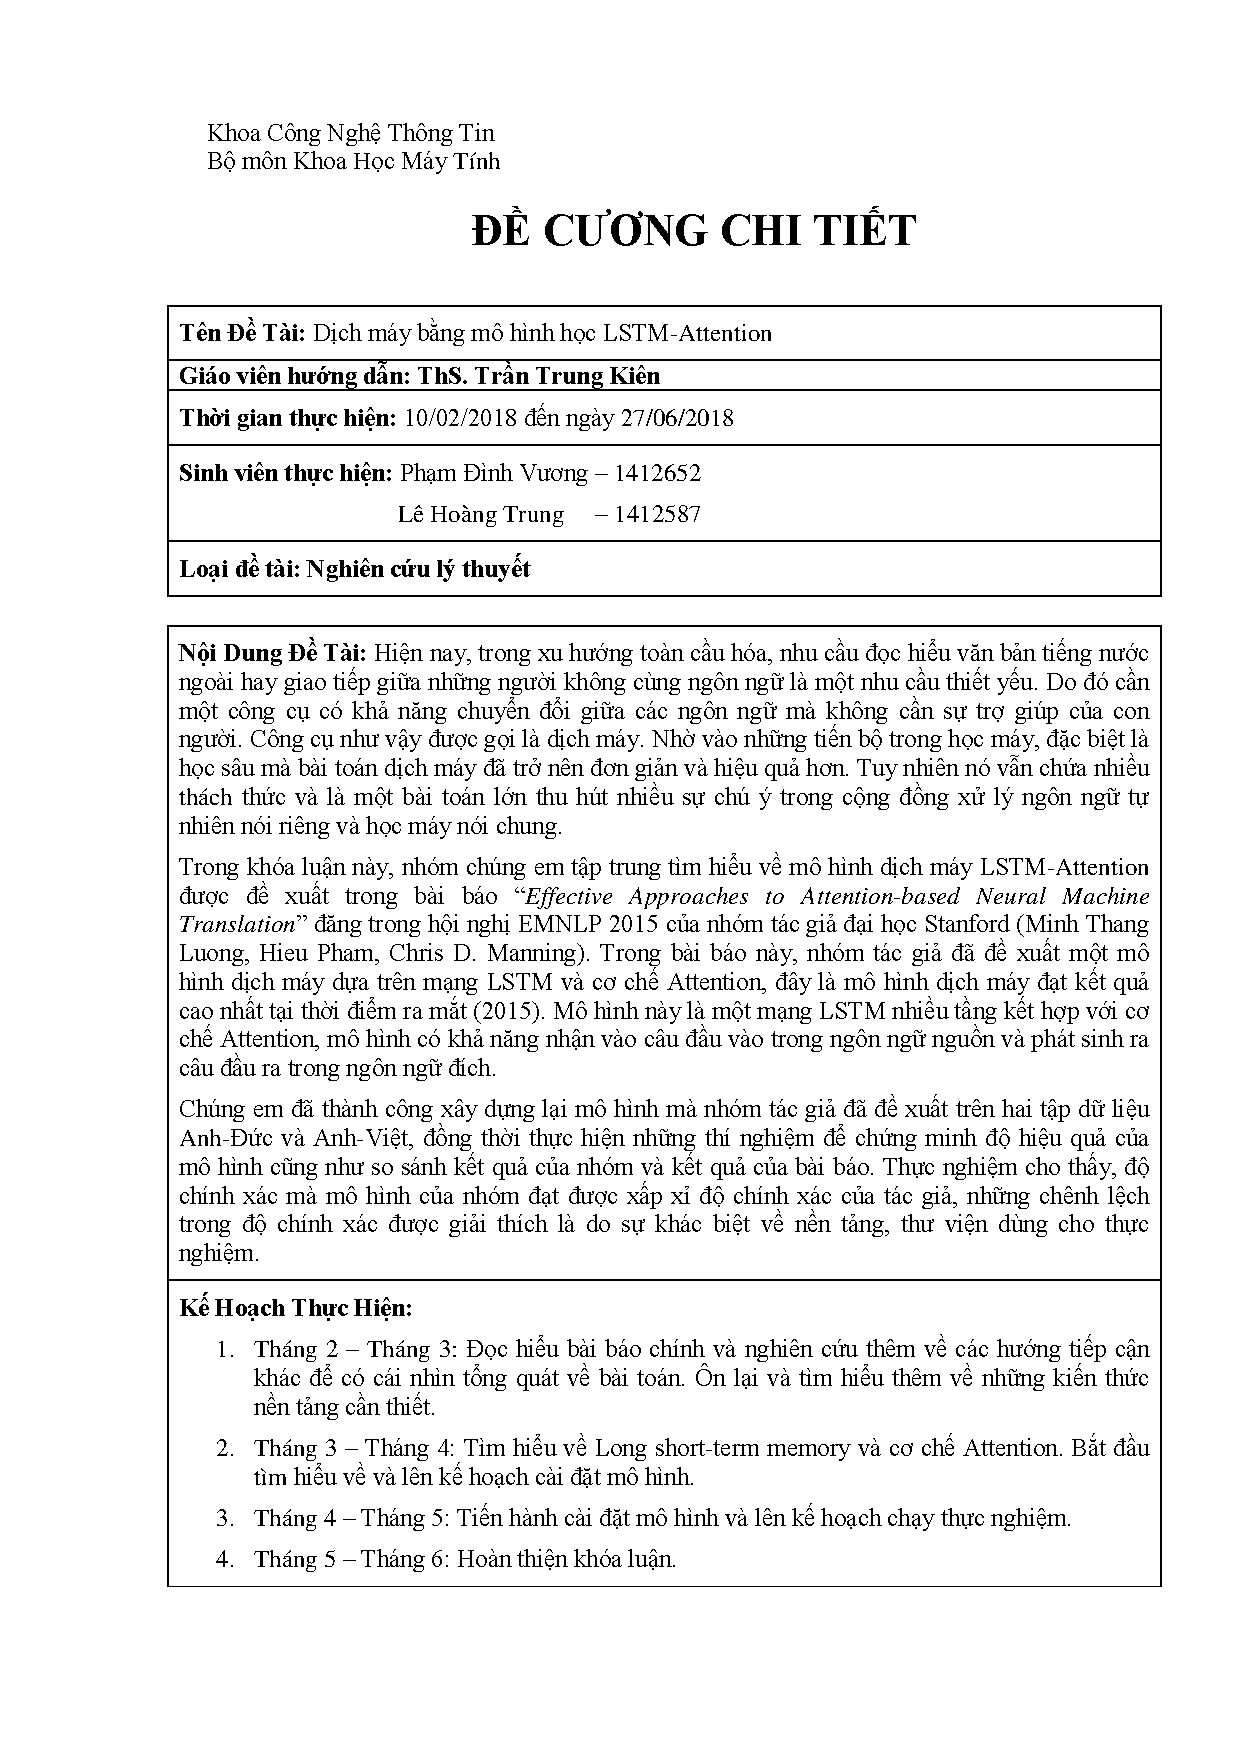
\includepdf[pages=1-2,pagecommand=\thispagestyle{plain}]{docs/DeCuongChiTiet}
	
	%\newpage
\chapter*{TÓM TẮT}
\addcontentsline{toc}{chapter}{TÓM TẮT} 

 Việc nghiên cứu, xây dựng các thuật toán chất lượng cao để giúp máy tính mô hình hóa, giải thích các hoạt động của con người là một vấn đề ngày càng được quan tâm và đầu tư hơn. Về tổng quan, các mô hình tự động nhận dạng hành động người có tiềm năng ứng dụng rất cao trong thực tế, như: truy vấn video, phân tích hành vi của bệnh nhân trong chẩn đoán bệnh, giám sát an ninh (chống ăn trộm, đánh nhau...), điều khiển video games thông qua cử chỉ và nhiều hệ thống tương tác ngưới-máy khác. Có thể nói, việc đưa ra một giải pháp tổng quát giúp máy hiểu được mọi cử chỉ, hành vi của con người vẫn đang là một bài toán đầy thách thức đối với cộng đồng nghiên cứu, bất chấp những nổ lực rất lớn đã được thực hiện qua hàng thập kỷ.
 
 Sự bùng nổ của công nghệ camera 3 chiều giá thành thấp (như Kinect) trong những năm gần đây đã mở ra nhiều giải pháp giúp đơn giản hóa các tác vụ nhận dạng hành động phức tạp, trong khi vẫn có thể đảm bảo được tiêu chí về tốc độ xử lý thời gian thực. Hòa nhịp cùng với xu hướng nghiên cứu hiện nay, khóa luận tập trung vào giải lớp bài toán nhận dạng hành động người trên dữ liệu đa phương thức RGB-D(gồm thông tin màu và độ sâu) thu được từ Kinect. Trên cơ sở lấy cảm hứng từ các giả thuyết về sự kích thích thị giác ở người tại các vùng nổi bật (\textit{visual attention}), khóa luận tiếp cận theo hướng khai thác các đặc trưng ngữ nghĩa, đặc thù với từng kênh dữ liệu màu-độ sâu, qua đó đề xuất một mô hình kết hợp hiệu quả các thông tin này để biểu diễn và phân lớp các hành động trên video. 

Kết quả sơ bộ mà khóa luận đạt được cho thấy việc trích chọn, kết hợp thông tin đặc trưng từ nhiều kênh dữ liệu như màu-độ sâu là rất cần thiết để tăng cường tri thức cho các hệ thống nhận dạng hành động người. Qua đó, giải pháp trình bày trong khóa luận cũng mở ra một hướng đi hứa hẹn trên con đường giúp máy tính có thể tiến gần hơn tới năng lực nhận thức và cảm thụ thị giác của con người.  
%	Hệ thị giác của người có thể cảm nhận được các cảnh liên tục, nhận biết sự vật và nắm bắt ngữ nghĩa chuyển động dễ dàng. Các nhà thần kinh, tâm lý học đã cố gắng phân tích và giải thích cơ chế giúp hệ thị giác người có thể hoạt động chính xác. Một số lý thuyết / giả thuyết như sự kích thích thị giác tại các vùng nổi bật (\textit{visual attention}), các luật "Gestalt" về cách tổ chức nhận thức đã được đặt ra, giải thích và làm sáng tỏ. Trên cơ sở lấy cảm hứng từ các thuật toán học dựa vào việc phân tích các đặc trưng thị giác nổi bật, chúng tôi cố gắng mô hình hóa và tích hợp các khám phá nhận thức thị giác quan trọng vào một hệ thống nhận dạng cử chỉ tổng quát. Đây cũng là một thành phần cơ bản, quan trọng trong mô hình tổng thể mà chúng ta đang hướng tới – một mô hình chung có thể học và hiểu mọi hoạt động, hành vi của con người.

	
	\newpage
	\renewcommand{\contentsname}{\centerline{MỤC LỤC}}
	\addcontentsline{toc}{chapter}{MỤC LỤC}
	\tableofcontents
	
	\newpage
	\renewcommand\listfigurename{\centerline{DANH MỤC HÌNH ẢNH}}
	\addcontentsline{toc}{chapter}{DANH MỤC HÌNH ẢNH}
	\listoffigures
	
	
	\newpage
	\renewcommand\listtablename{\centerline{DANH MỤC BẢNG}}
	\addcontentsline{toc}{chapter}{DANH MỤC BẢNG}
	\listoftables
	%
	%\newpage
	%\renewcommand{\nomname}{
	%	\addcontentsline{toc}{chapter}{DANH MỤC THUẬT NGỮ VIẾT TẮT}
	%	{\fontsize{25}{25}\selectf>>>>>>> origin/attentionont
	%	DANH MỤC THUẬT NGỮ VIẾT TẮT}
	%	}	
	%%\makeglossaries
	%\nomenclature{$STIP:$}{Space-Time Interest Points - Điểm trọng yếu không-thời gian}
	%\nomenclature{$SC:$}{Sparse Coding}
	%\nomenclature{$BoF:$}{Bag of Feature - Giỏ đặc trưng}
	%\nomenclature{$HOG:$}{Histogram of Oriented Gradients - Lược đồ phân bố cường độ hướng biến thiên độ xám}
	%\nomenclature{$HONV:$}{Histogram of Oriented Normal Vectors - Lược đồ phân bố hướng của các vector pháp tuyến}
	%\nomenclature{$HOF:$}{Histogram of Optical Flows - Lược đồ phân bố 1luồng chuyển động}
	%\nomenclature{$3DS-HONV:$}{3D Spherical-Histogram of Oriented Nomal Vectors}
	%\nomenclature{$SVM:$}{Support Vector Machine - Bô phân lớp "Máy hỗ trợ vector"}
	%\nomenclature{$kNN:$}{k Nearest Neighbors - k láng giềng gần nhất}
	%\nomenclature{$Confusion:$}{Ma trận nhầm lẫn - dùng để mô tả số kết quả phân loại đúng và sai tại mỗi lớp(class)}
	%\nomenclature{$DTW:$}{Dynamic Time Warping - thuật toán so khớp các chuỗi tín hiệu tương tự theo thời gian}
	%\nomenclature{$R.O.I: $}{Region of Interest - Vùng ứng viên hay Vùng quan tâm}
	%\nomenclature{$TGMT: $}{Thị giác máy tính}
	%%\printglossary[type=\acronymtype,title=Abbreviations]
	%\printnomenclature[7em]
	%
	%\newpage
	%%\newglossaryentry{acr_norm}{
	%%  name = $\left\| \right\|$ ,
	%%  description = Phép tính norm,
	%%}
	%\newglossaryentry{acr_concate}{
	%  name = $\odot\hspace{0.2in}$ ,
	%  description = Phép nối 2 vector đặc trưng
	%}
	%\newglossaryentry{acr_early_fusion}{
	%  name = $A-B\hspace{0.2in}$ ,
	%  description = Phép kết hợp trước 2 vector đặc trưng A và B (early fusion)
	%}
	%\newglossaryentry{acr_late_fusion}{
	%  name = $A/B\hspace{0.2in}$ ,
	%  description = Phép kết hợp trễ 2 vector đặc trưng A và B (late fusion)
	%}
	%\newglossaryentry{acr_st}{
	%  name = $s.t.\hspace{0.1in}$ ,
	%  description = thỏa điều kiện (subject to)
	%}
	%\newglossaryentry{acr_hist}{
	%  name = $hist\hspace{0.1in}$ ,
	%  description = Lược đồ phân bố (histogram)
	%}
	%\makeglossaries
	%
	%\printglossary[title=KÝ HIỆU - QUY ƯỚC]{\addcontentsline{toc}{chapter}{KÝ HIỆU-QUY ƯỚC}}
	
	
	%\input{Abstract}
	\newpage
	\pagenumbering{arabic}
	
	% define softmax - Trung
	\newcommand\softmax[0]{\mathrm{softmax}}
	
	% \pagebreak[4]
% \hspace*{1cm}
% \pagebreak[4]
% \hspace*{1cm}
% \pagebreak[4]

\chapter{Giới thiệu }
\ifpdf
    \graphicspath{{Chapter1/Chapter1Figs/PNG/}{Chapter1/Chapter1Figs/PDF/}{Chapter1/Chapter1Figs/}}
\else
    \graphicspath{{Chapter1/Chapter1Figs/EPS/}{Chapter1/Chapter1Figs/}}
\fi

Nhờ vào những cải cách trong giao thông và cơ sở hạ tầng viễn thông mà giờ đây toàn cầu hóa đang trở nên gần với chúng ta hơn bao giờ hết. Trong xu hướng đó nhu cầu giao tiếp và thông hiểu giữa những nền văn hóa là không thể thiếu. Tuy nhiên, những nền văn hóa khác nhau thường kèm theo đó là sự khác biệt về ngôn ngữ, là một trong những trở ngại lớn nhất của sự giao tiếp. Một người phải mất rất nhiều thời gian để thành thạo một ngôn ngữ không phải là tiếng mẹ đẻ, và không thể nào học được nhiều ngôn ngữ cùng lúc. Cho nên, việc phát triển một công cụ để giải quyết vấn đề này là tất yếu. Một trong những công cụ như vậy là \textit{Dịch máy}.

\textit{Dịch máy} là quá trình chuyển đổi văn bản/tiếng nói từ ngôn ngữ này sang dạng tương ứng của nó trong một ngôn ngữ khác, được thực hiện bởi một chương trình máy tính nhằm mục đích cung cấp bản dịch tốt nhất mà không cần sự trợ giúp của con người.

Dịch máy có một quá trình lịch sử lâu dài. Từ thế kỷ XVII, đã có những ý tưởng về việc cơ giới hóa quá trình dịch thuật. Tuy nhiên, đến thế kỷ XX, những nghiên cứu về dịch máy mới thật sự bắt đầu. Vào những năm 1930, Georges Artsrouni người Pháp và Petr Troyanskii người Nga đã nộp bằng sáng chế cho công trình có tên "máy dịch" của riêng họ. Trong số hai người, công trình của Troyanskii có ý nghĩa hơn. Nó đề xuất không chỉ một phương pháp cho bộ từ điển tự động, mà còn là lược đồ cho việc mã hóa các vai trò ngữ pháp song ngữ và một phác thảo về cách phân tích và tổng hợp có thể hoạt động. Tuy nhiên, những ý tưởng của Troyanskii đã không được biết đến cho đến cuối những năm 1950. Trước đó, máy tính đã được phát minh.

Những nỗ lực xây dựng hệ thống dịch máy bắt đầu ngay sau khi máy tính ra đời. Có thể nói, chiến tranh và sự thù địch giữa các quốc gia là động lực lớn nhất cho dịch máy thời bấy giờ. Trong Thế chiến thứ II, máy tính đã được quân đội Anh sử dụng trong việc giải mã các thông điệp được mã hóa của quân Đức. Việc làm này có thể coi là một dạng ẩn dụ của dịch máy khi người ta cố gắng dịch từ tiếng Đức được mã hóa sang tiếng Anh. Trong thời kỳ chiến tranh lạnh, vào tháng 7/1949, Warren Weaver, người được xem là nhà tiên phong trong lĩnh vực dịch máy, đã viết một bản ghi nhớ đưa ra các đề xuất khác nhau của ông trong lĩnh vực này. Những đề xuất đó dựa trên thành công của máy phá mã, sự phát triển của lý thuyết thông tin bởi Claude Shannon và suy đoán về các nguyên tắc phổ quát cơ bản của ngôn ngữ. Trong vòng một năm, một vài nghiên cứu về dịch máy đã bắt đầu tại nhiều trường đại học của Mỹ. Vào ngày 7/1/1954, tại trụ sở chính của IBM ở New York, thử nghiệm Georgetown-IBM được tiến hành. Máy tính IBM 701 đã tự động dịch 49 câu tiếng Nga sang tiếng Anh lần đầu tiên trong lịch sử chỉ sử dụng 250 từ vựng và sáu luật ngữ pháp \cite{hutchins}. Thí nghiệm này được xem như là một thành công và mở ra kỉ nguyên cho những nghiên cứu với kinh phí lớn về dịch máy ở Hoa Kỳ. Ở Liên Xô những thí nghiệm tương tự cũng được thực hiện không lâu sau đó.

Trong một thập kỷ tiếp theo, nhiều nhóm nghiên cứu về dịch máy được thành lập. Một số nhóm chấp nhận phương pháp thử và sai, thường dựa trên thống kê với mục tiêu là một hệ thống dịch máy có thể hoạt động ngay lập tức, tiêu biểu như: nhóm nghiên cứu tại đại học Washington (và sau này là IBM) với hệ thống dịch Nga-Anh cho Không quân Hoa Kỳ, những nghiên cứu tại viện Cơ học Chính xác ở Liên Xô và Phòng thí nghiệm Vật lý Quốc gia ở Anh. Trong khi một số khác hướng đến giải pháp lâu dài với hướng tiếp cận lý thuyết bao gồm cả những vấn đề liên quan đến ngôn ngữ cơ bản như nhóm nghiên cứu tại Trung tâm nghiên cứu lý thuyết tại MIT, Đại học Havard và Đơn vị nghiên cứu ngôn ngữ Đại học Cambridge. Những nghiên cứu trong giai đoạn này có tầm quan trọng và ảnh hưởng lâu dài không chỉ cho Dịch máy mà còn cho nhiều ngành khác như Ngôn ngữ học tính toán, Trí tuệ nhân tạo - cụ thể là việc phát triển các từ điển tự động và kỹ thuật phân tích cú pháp. Nhiều nhóm nghiên cứu đã đóng góp đáng kể cho việc phát triển lý thuyết ngôn ngữ. Tuy nhiên, mục tiêu cơ bản của dịch máy là xây dựng hệ thống có khả năng tạo ra bản dịch tốt lại không đạt được dẫn đến một kết quả là vào năm 1966 bản báo cáo từ Ủy ban tư vấn xử lý ngôn ngữ tự động (Automatic Language Processing Advisory) của Hoa Kỳ, tuyên bố rằng dịch máy là đắt tiền, không chính xác và không mang lại kết quả hứa hẹn \cite{hutchins}. Thay vào đó, họ đề nghị tập trung vào phát triển các từ điển, điều này đã loại bỏ các nhà nghiên cứu Mỹ ra khỏi cuộc đua trong gần một thập kỷ.

\begin{figure}
	\centering
	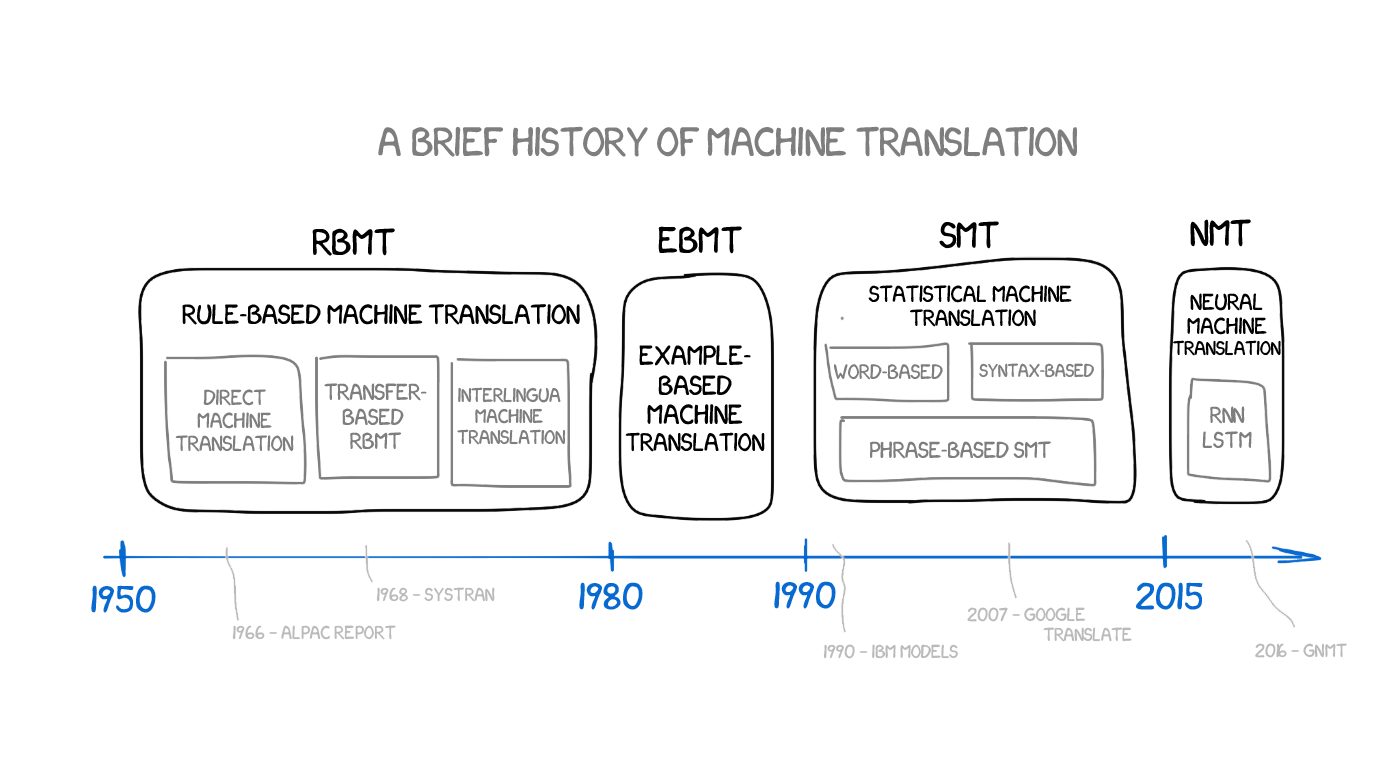
\includegraphics[width=\textwidth]{mthistory}
	\caption[Lịch sử tóm tắt của dịch máy]{Lịch sử tóm tắt của dịch máy, nguồn ảnh: Ilya Pestov trong blog \href{https://medium.freecodecamp.org/a-history-of-machine-translation-from-the-cold-war-to-deep-learning-f1d335ce8b5}{A history of machine translation from the Cold War to deep learning}}
	\label{fig_mthistory}
\end{figure}

\section{Các phương pháp Dịch máy}

Từ đó đến nay, đã có nhiều hướng tiếp cập đã được sử dụng trong dịch máy với mục tiêu tạo ra bản dịch có độ chính xác cao và giảm thiểu công sức của con người. Trong những năm đầu tiên, để tạo ra bản dịch tốt, các phương pháp thời bấy giờ đều hỏi hỏi những lý thuyết tinh vi về ngôn ngữ học. Hầu hết những hệ thống dịch máy trước những năm 1980 đều là \textit{dịch máy dựa trên luật (Rule-based machine translation - RBMT)}. Những hệ thống này thường bao gồm:
\begin{itemize}
	\item[•] Một từ điển song ngữ (ví dụ từ điển Anh - Đức)
	\item[•] Một tập các luật ngữ pháp (ví dụ trong tiếng Đức, từ kết thúc bằng -heit, -keit, -ung là những từ mang giống cái)		
\end{itemize} 

\begin{figure}
	\centering
	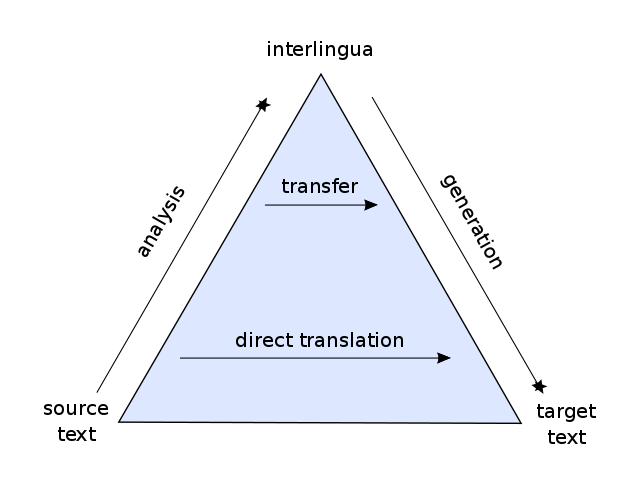
\includegraphics[width=0.5\textwidth]{rulebasedpyramid}
	\caption[Ba phương pháp dịch máy dựa trên luật]{Kim tự tháp của Bernard Vauquois thể hiện ba phương pháp dịch máy dựa luật theo độ sâu của đại diện trung gian. Bắt đầu từ dịch máy trực tiếp đến dịch máy chuyển dịch và trên cùng là dịch máy ngôn ngữ phổ quát (Nguồn: \href{http://en.wikipedia.org/wiki/Machine_translation}{http://en.wikipedia.org/wiki/Machine\_translation})}
	\label{fig_rulebasedpyramid}
\end{figure}

Có ba cách tiếp cận khác nhau theo phương pháp dịch máy dựa trên luật. Bao gồm phương pháp dịch máy trực tiếp, dịch máy chuyển giao và dịch máy ngôn ngữ phổ quát. Mặc dù cả ba đều thuộc về RBMT, tuy nhiên chúng khác nhau về độ sâu của đại diện trung gian. Sự khác biệt này được thể hiện qua kim tự tháp Vauquois, minh họa trên hình \ref{fig_rulebasedpyramid} 
%\begin{itemize}
%	\item[•] \textit{Dịch máy trực tiếp} (Direct machine translation - DMT): Đây là phương pháp đơn giản nhất của dịch máy. DMT không dùng bất cứ dạng đại diện nào của ngôn ngữ nguồn, nó chia câu thành các từ, dịch chúng bằng một từ điển song ngữ. Sau đó, dựa trên các luật mà những nhà ngôn ngữ học đã xây dựng, nó chỉnh sửa để bản dịch trở nên đúng cú pháp và ít nhiều đúng về mặt phát âm.
%	\item[•] \textit{Dịch máy ngôn ngữ phổ quát} (Interlingual machine translation - IMT): Trong phương pháp này, câu nguồn được chuyển thành biểu diễn trung gian và biểu diễn này được thống nhất cho tất cả ngôn ngữ trên thế giới (interlingua). Tiếp theo, dạng đại diện này sẽ được chuyển đổi sang bất kỳ ngôn ngữ đích nào. Một trong những ưu điểm chính của hệ thống này là tính mở rộng của nó khi số lượng ngôn ngữ cần dịch tăng lên. Mặc dù trên lý thuyết, phương pháp này trông rất hoàn hảo. Nhưng trong thực tế, thật khó để tạo được một ngôn ngữ phổ quát như vậy.
%	\item[•] \textit{Dịch máy chuyển giao} (Transfer-based machine translation - TMT): dịch máy chuyển giao tương tự như dịch máy ngôn ngữ đại diện ở chỗ, nó cũng tạo ra bản dịch từ biểu diễn trung gian mô phỏng ý nghĩa của câu gốc. Không giống như IMT, TMT phụ thuộc một phần vào cặp ngôn ngữ mà nó tham gia vào quá trình dịch. Trên cơ sở sự khác biệt về cấu trúc của ngôn ngữ nguồn và ngôn ngữ đích, một hệ thống TMT có thể được chia thành ba giai đoạn: i) Phân tích, ii) Chuyển giao, iii) Tạo ra bản dịch. Trong giai đoạn đầu tiên, trình phân tích cú pháp ở ngôn ngữ nguồn được sử dụng để tạo ra biểu diễn cú pháp của câu nguồn. Trong giai đoạn tiếp theo, kết quả của phân tích cú pháp được chuyển đổi thành biểu diễn tương đương trong ngôn ngữ đích. Trong giai đoạn cuối cùng, một bộ phân tích hình thái của ngôn ngữ đích được sử dụng để tạo ra các bản dịch cuối cùng.
%\end{itemize}

\textit{Dịch máy trực tiếp} (Direct machine translation - DMT): Đây là phương pháp đơn giản nhất của dịch máy. DMT không dùng bất cứ dạng đại diện nào của ngôn ngữ nguồn, nó chia câu thành các từ, dịch chúng bằng một từ điển song ngữ. Sau đó, dựa trên các luật mà những nhà ngôn ngữ học đã xây dựng, nó chỉnh sửa để bản dịch trở nên đúng cú pháp và ít nhiều đúng về mặt phát âm.

\textit{Dịch máy ngôn ngữ phổ quát} (Interlingual machine translation - IMT): Trong phương pháp này, câu nguồn được chuyển thành biểu diễn trung gian và biểu diễn này được thống nhất cho tất cả ngôn ngữ trên thế giới (interlingua). Tiếp theo, dạng đại diện này sẽ được chuyển đổi sang bất kỳ ngôn ngữ đích nào. Một trong những ưu điểm chính của hệ thống này là tính mở rộng của nó khi số lượng ngôn ngữ cần dịch tăng lên. Mặc dù trên lý thuyết, phương pháp này trông rất hoàn hảo. Nhưng trong thực tế, thật khó để tạo được một ngôn ngữ phổ quát như vậy.

\textit{Dịch máy chuyển giao} (Transfer-based machine translation - TMT): dịch máy chuyển giao tương tự như dịch máy ngôn ngữ đại diện ở chỗ, nó cũng tạo ra bản dịch từ biểu diễn trung gian mô phỏng ý nghĩa của câu gốc. Tuy nhiên, không giống như IMT, TMT phụ thuộc một phần vào cặp ngôn ngữ mà nó tham gia vào quá trình dịch. Trên cơ sở sự khác biệt về cấu trúc của ngôn ngữ nguồn và ngôn ngữ đích, một hệ thống TMT có thể được chia thành ba giai đoạn: i) Phân tích, ii) Chuyển giao, iii) Tạo ra bản dịch. Trong giai đoạn đầu tiên, trình phân tích cú pháp ở ngôn ngữ nguồn được sử dụng để tạo ra biểu diễn cú pháp của câu nguồn. Trong giai đoạn tiếp theo, kết quả của phân tích cú pháp được chuyển đổi thành biểu diễn tương đương trong ngôn ngữ đích. Trong giai đoạn cuối cùng, một bộ phân tích hình thái của ngôn ngữ đích được sử dụng để tạo ra các bản dịch cuối cùng.

Mặc dù đã có một số hệ thống RBMT được đưa vào sử dụng như PROMPT \cite{promt} và Systrans \cite{systrans}. Tuy nhiên, bản dịch của hướng tiếp cận này có chất lượng thấp so với nhu cầu của con người và không sử dụng được trừ một số trường hợp đặc biệt. Ngoài ra chúng còn có một số nhược điểm lớn như:
\begin{itemize}
	\item[•] Các loại từ điển chất lượng tốt có sẵn là không nhiều và việc xây dựng những bộ từ điển mới là rất tốn kém.
	\item[•] Hầu hết những luật ngôn ngữ được tạo ra bằng tay bởi các nhà ngôn ngữ học. Việc này gây khó khăn và tốn kém khi hệ thống trở nên lớn hơn.
	\item[•] Các hệ thống RBMT gặp khó khăn trong việc giải quyết những vấn đề như thành ngữ hay sự nhập nhằng về ngữ nghĩa của các từ. 
\end{itemize}
Từ những năm 1980, dịch máy dựa trên \textit{Ngữ liệu} (Corpus-based machine translation) được đề xuất. Điểm khác biệt lớn nhất và cũng là quan trọng nhất của hướng tiếp cận này so với RBMT là thay vì sử dụng các bộ từ điển song ngữ, nó dùng những tập câu tương đương trong hai ngôn ngữ làm nền tảng cho việc dịch thuật. Tập những câu tương đương này được gọi là ngữ liệu. So với từ điển, việc thu thập ngữ liệu đơn giản hơn rất nhiều. Ví dụ như ta có thể tìm thấy nhiều phiên bản trong các ngôn ngữ khác nhau của những văn bản hành chính hay các trang web đa ngôn ngữ. Trước khi dịch máy nơ-ron ra đời, dịch máy dựa trên ngữ liệu bao gồm hai phương pháp: dịch máy dựa trên ví dụ và dịch máy thống kê.

%Nhóm thứ hai là những hướng tiếp cận dựa trên \textit{Ngữ liệu} (Corpus based). Nhóm này hoạt động dựa trên một tập dữ liệu song song của các cặp câu là bản dịch của nhau trong hai ngôn ngữ gọi là ngữ liệu và chỉ yêu cầu những tri thức tối thiểu về ngôn ngữ học. Trước khi dịch máy nơ-ron ra đời, phương pháp nổi bật và hiệu quả nhất dựa trên hướng tiếp cận này chính là \textit{Dịch máy thống kê} (Statistical machine translation). Vào năm 1990, IBM công bố hệ thống dịch máy thống kê của họ, đây là hệ thống đầu tiên có khả năng tạo ra bản dịch mà không cần biết gì về các từ hay quy tắc ngữ pháp của ngôn ngữ. Chỉ cần cung cấp bộ ngữ liệu, hệ thống này phân tích các câu tương ứng trong ngữ liệu đó để hiểu được các mô hình bên dưới.
\textit{Dịch máy dựa trên ví dụ} (Example-based Machine Translation - EBMT): 

\textit{Dịch máy thống kê} (Statistical machine translation - SMT): ý tưởng của phương pháp này là thay vì định nghĩa những từ điển và các luật ngữ pháp một cách thủ công, SMT dùng mô hình thống kê để học các từ điển và các luật ngữ pháp này từ ngữ liệu. Những ý tưởng đầu tiên của SMT được giới thiệu đầu tiên bởi Waren Weaver vào năm 1949 bap gồm việc áp dụng lý thuyết thông tin của Claude Shannon vào dịch máy. SMT được giới thiệu lại vào cuối những năm 1980 và đầu những năm 1990 tại trung tâm nghiên cứu Thomas J. Watson của IBM. SMT là phương pháp được nghiên cứu rộng rãi nhất thời bấy giờ và thậm chí đến hiện tại, nó vẫn là một trong những phương pháp được nghiên cứu nhiều nhất về dịch máy. 

Để hiểu rõ hơn về dịch máy thống kê, xét một ví dụ: ta cần dịch một câu $f$ trong tiếng Pháp sang dạng tiếng Anh $e$ của nó. Có nhiều bản dịch có thể có cuả $f$ trong tiếng Anh, việc cần làm là chọn $e$ sao cho nó là bản dịch "tốt nhất" của $f$. Chúng ta có thể mô hình hóa quá trình này bằng một xác suất có điều kiện $P(e|f)$ với $e$ là những bản dịch có thể có với câu cho trước $f$. Một cách hợp lý để chọn bản dịch "tốt nhất" là chọn $e$ sao cho nó tối đa xác suất có điều kiện $p(e|f)$. Cách tiếp cận quen thuộc là sử dụng định lý Bayes để viết lại $p(e|f)$:
\begin{equation} \label{bayesFomular}
	p(e|f) = \frac{p(f|e)p(e)}{p(f)}
\end{equation}
Bởi vì $f$ là cố định, tối đa hóa $p(e|f)$ tương đương với tìm $e$ sao cho tối đa hóa $p(f|e)p(e)$. Để làm được điều này, chúng ta dựa vào một tập ngữ liệu là những câu song ngữ Anh - Pháp để suy ra các mô hình $P(f|e)$ và $P(e)$ và sử dụng những mô hình đó để tìm một bản dịch cụ thể $\tilde{e}$ sao cho:
\begin{equation} \label{ehatSMT}
	\tilde{e} = \arg\max_{e \in e^*} p(e|f) = \arg\max_{e \in e^*} p(f|e)p(e)
\end{equation}
Ở đây, $p(f|e)$ được gọi là \textit{mô hình dịch} (translation model) và $p(e)$ được gọi là \textit{mô hình ngôn ngữ} (language model). Mô hình dịch $p(f|e)$ thể hiện khả năng câu $e$ là một bản dịch của câu $f$. Những mô hình dịch ban đầu dựa trên từ (word-based) như các mô hình IBM 1-5 (IBM Models 1-5). Những năm 2000, những mô hình dịch dựa trên cụm từ (phrase based) xuất hiện giúp cải thiện khả năng dịch của SMT. Trong khi đó, mô hình ngôn ngữ $p(e)$ thể hiện độ trơn tru của câu $e$. Ví dụ $p($"tôi đi học"$) >$ $p($"học tôi đi"$)$ vì rõ ràng "tôi đi học" là có lý hơn "học tôi đi". Các mô hình ngôn ngữ cho SMT thường được ước lượng bằng các mô hình n-gram được làm mịn, cách làm này cũng là một nhược điểm của SMT. Mô hình ngôn ngữ là một chủ đề quan trọng và sẽ được chúng tôi đề cập lại một lần nữa trong chương Kiến thức nền tảng.

\begin{figure}
	\centering
	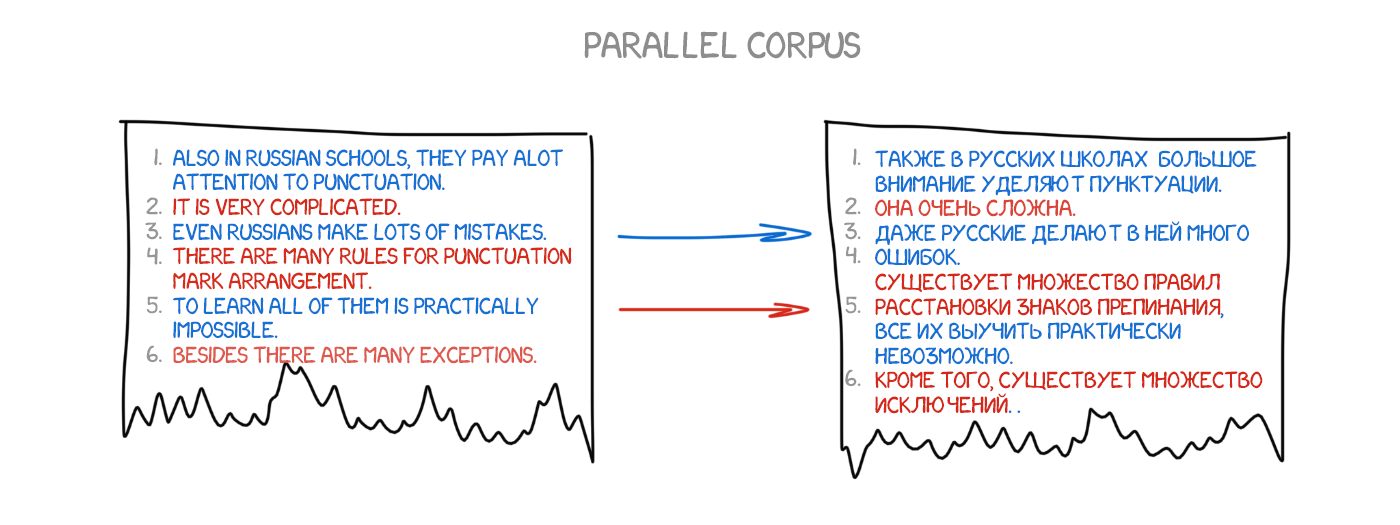
\includegraphics[width=\textwidth]{smt}
	\caption[Ví dụ về tập các câu song song trong hai ngôn ngữ]{Ví dụ về tập các câu song song trong hai ngôn ngữ}
	\label{fig_parallelcorpus}
\end{figure}


\section{Dịch máy Nơ-ron}

Mặc dù trên thực tế đã có nhiều hệ thống dịch máy được phát triển dựa trên dịch máy thống kê thời bấy giờ, tuy nhiên nó không hoạt động thực sự tốt bởi một số nguyên nhân. Một là việc những từ hay đoạn được dịch cục bộ và quan hệ của chúng với những từ cách xa trong câu nguồn thường bị bỏ qua. Hai là mô hình ngôn ngữ N-gram hoạt động không thực sự tốt đối với những bản dịch dài và ta phải tốn nhiều bộ nhớ để lưu trữ chúng. Ngoài ra việc sử dụng nhiều thành phần nhỏ được điều chỉnh riêng biệt như mô hình dịch, mô hình ngôn ngữ,.. cũng gây khó khăn cho việc vận hành và phát triển mô hình này.

% TODO: Kalchbrenner and Blunsom (2013), Sutskever et al. (2014) and Cho et al. (2014b)
\textit{Dịch máy nơ-ron} (Neural machine translation) là một hướng tiếp cận mới trong dịch máy trong những năm gần đây được đề xuất đầu tiên bởi \cite{kalchbrennerBlunsom}, \cite{sutskever}, \cite{cho}. Giống như dịch máy thống kê, dịch máy nơ-ron cũng là một phương pháp thuộc hướng tiếp cận dựa trên ngữ liệu, trong khi dịch máy thống kê bao gồm nhiều mô-đun nhỏ được điều chỉnh riêng biệt, Dịch máy nơ-ron cố gắng dùng một mạng nơ-ron như là thành phần duy nhất của hệ thống, mọi thiết lập sẽ được thực hiện trên mạng này. 

% TODO: Sutskever et al., 2014; Cho et al., 2014a
Hầu hết những mô hình dịch máy nơ-ron đều dựa trên kiến trúc \textit{Bộ mã hóa - Bộ giải mã} (Encoder-Decoder) (\cite{sutskever}, \cite{cho}). Bộ mã hóa thường là một mạng nơ-ron có tác dụng \textit{"nén"} tất cả thông tin của câu trong ngôn ngữ nguồn vào một vector có kích thước cố định. Bộ giải mã, cũng là một mạng nơ-ron, sẽ tạo bản dịch trong ngôn ngữ đích từ vector có kích thước cố định kia. Toàn bộ hệ thống bao gồm bộ mã hóa và bộ giải mã sẽ được huấn luyện \textit{"end-to-end"} để tạo ra bản dịch, quá trình này được mô tả như hình 1.2.

\begin{figure}
	\centering
	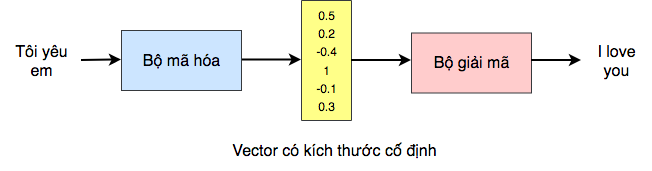
\includegraphics[width=\textwidth]{intro2nmt}
	\caption[Ví dụ về Kiến trúc \textit{bộ mã hóa - bộ giải mã} trong dịch máy nơ-ron]{Ví dụ về kiến trúc bộ mã hóa - bộ giải mã trong dịch máy nơ-ron}
	\label{fig_encoder_decoder}
\end{figure}

% TODO: mention LSTM
Trong thực tế cả bộ mã hóa và giải mã thường dựa trên một mô hình mạng nơ-ron tên là \textit{Mạng nơ-ron hồi quy} là một thiết kế mạng đặc trưng cho việc xử lý dữ liệu chuỗi. Mạng nơ-ron hồi quy cho phép chúng ta mô hình hóa những dữ liệu có độ dài không xác định, rất thích hợp cho bài toán dịch máy. Hình 1.3 mô tả chi tiết hơn về kiến trúc bộ mã hóa - giải mã sử dụng mạng nơ-ron hồi quy. Đầu tiên bộ mã hóa đọc qua toàn bộ câu nguồn và tạo ra một vector đại diện gọi là \textit{vector trạng thái}. Điều này giúp cho toàn bộ những thông tin cần thiết hay quan hệ giữa các từ đều được tập hợp vào một nơi duy nhất. Bộ giải mã, lúc này đóng vai trò như một mô hình ngôn ngữ để tạo ra từng từ trong ngôn ngữ đích và sẽ dừng lại đến khi một ký tự đặc biệt xuất hiện.

\begin{figure}
	\centering
	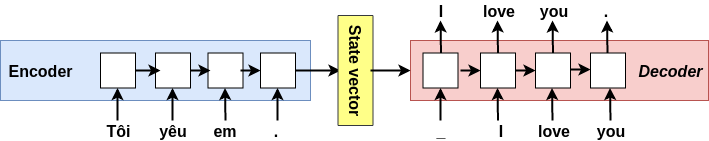
\includegraphics[width=\textwidth]{encoder-decoder}
	\caption[Kiến trúc bộ mã hóa - bộ giải mã được xây dựng trên mạng nơ-ron hồi quy]{Kiến trúc bộ mã hóa - bộ giải mã được xây dựng trên mạng nơ-ron hồi quy}
	\label{fig_encoder_decoder_details}
\end{figure}

Trong hình 2, có thể thấy rằng bộ giải mã tạo ra bản dịch chỉ dựa trên trạng thái ẩn cuối cùng, cũng chính là vector có kích thước cố định được tạo ra ở bộ mã hóa. Vector này phải mã hóa mọi thứ chúng ta cần biết về câu nguồn. Giả sử chúng ta có câu nguồn với độ dài là 50 từ, từ đầu tiên ở câu đích có lẽ sẽ có mối tương quan cao với từ đầu tiên ở câu nguồn. Điều này có nghĩa là bộ giải mã phải xem xét thông tin được mã hóa từ 50 \textit{"time step"} trước đó. Mạng nơ-ron hồi quy được chứng minh là gặp khó khăn trong việc mã hóa những chuỗi dài \cite{difficultyRNN}. Để giải quyết vấn đề này, thay vì dùng mạng nơ-ron hồi quy thuần, người ta sử dụng các biến thể của nó quy như \textit{Long short-term memory (LSTM)}. Trên lý thuyết, LSTM có thể giải quyết vấn đề mất mát thông tin trong chuỗi dài, nhưng trong thực tế vấn đề này vẫn chưa thể được giải quyết hoàn toàn. Một số nhà nghiên cứu đã phát hiện ra rằng đảo ngược chuỗi nguồn trước khi đưa vào bộ mã hóa tạo ra kết quả tốt hơn một cách đáng kể \cite{sutskever} bởi nó khiến cho những từ đầu tiên được đưa vào bộ mã hóa sau cùng, và được giải mã thành từ tương ứng ngay sau đó. Cách làm này tuy giúp cho bản dịch hoạt động tốt hơn trong thực tế, nhưng nó không phải là một giải pháp về mặt thuật toán. Hầu hết các đánh giá về dịch máy được thực hiện trên các ngôn ngữ như ngôn ngữ có trật tự câu tương đối giống nhau. Ví dụ trật tự dạng "chủ ngữ - động từ - vị ngữ" như tiếng Anh, Đức, Pháp hay Trung Quốc. Đối với dạng ngôn ngữ có một trật tự khác ví dụ "chủ ngữ - vị ngữ - động từ" như tiếng Nhật, đảo ngược câu nguồn sẽ không hiệu quả.

\textit{Attention} là cơ chế giải phóng kiến trúc bộ mã hóa - bộ giải mã khỏi nhược điểm chỉ sử dụng một vector có chiều dài cố định làm đại diện cho câu đầu vào. Ý tưởng chính của cơ chế này là ở mỗi thời điểm phát sinh các từ trong bản dịch, bộ giải mã sẽ "nhìn" vào các phần khác nhau của câu nguồn trong quá trình mã hóa. Quan trọng hơn, cơ chế này cho phép mô hình học được cách chọn những phần cần thiết để tập trung vào dựa trên câu nguồn và những gì mà bộ giải mã đã giải mã được.

\begin{figure}
	\centering
	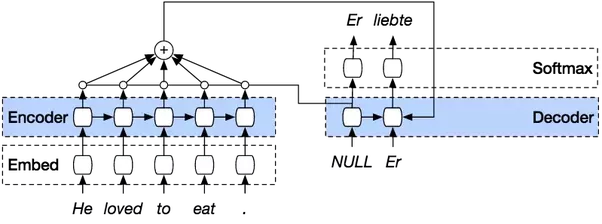
\includegraphics[width=\textwidth]{intro2attention}
	\caption[Cơ chế Attention trong dịch máy nơ-ron]{Cơ chế Attention trong dịch máy nơ-ron}
	\label{fig_introattention}
\end{figure} 

\section{Cấu trúc của khóa luận}
Trong khóa luận này, chúng tôi quyết định tập trung nghiên cứu về dịch máy nơ-ron và cơ chế Attention dựa trên nghiên cứu của nhóm tác giả tại đại học Stanford bao gồm Minh-Thang Luong, Hieu Pham, Christopher Manning trong bài báo \textit{Effective Approaches to Attention-based Neural Machine Translation} \cite{mainpaper}. Các phần còn lại trong luận văn được trình bày như sau:

\begin{itemize}
	\item[•] Chương 2 trình bày về những thành nền tảng của kiến trúc bộ mã hóa - giải mã
	
	\item[•] Chương 3 trình bày về cơ chế Attention, đây là phần chính của luận văn. Trong phần này gồm có hai phần nhỏ:
		\begin{itemize}
			\item[-] \textit{Global attetion}: là cơ chế tập trung vào tất cả các trạng thái ở câu nguồn
			\item[-] \textit{Local attetion}: tập trung vào một tập các trạng thái ở câu nguồn tại một thời điểm
		\end{itemize}
	\item[•] Chương 4 trình bày về các thí nghiệm và các phân tích về kết quả đạt trên hai tập dữ liệu Anh-Đức, Anh-Việt.
	\item[•] Kết luận và hướng phát triển của luận văn.
\end{itemize}






	\chapter{Kiến Thức Nền Tảng}
\ifpdf
    \graphicspath{{Chapter2/Chapter2Figs/PNG/}{Chapter2/Chapter2Figs/PDF/}{Chapter2/Chapter2Figs/}}
\else
    \graphicspath{{Chapter2/Chapter2Figs/EPS/}{Chapter2/Chapter2Figs/}}
\fi

\begin{quote}

Trong chương này, chúng tôi sẽ trình bày những kiến thức nền tảng trên ba chủ đề bao gồm mạng nơ-ron hồi quy, mô hình ngôn ngữ nơ-ron và mô hình dịch máy nơ-ron. Mạng nơ-ron hồi quy (RNN) là xương sống của dịch máy nơ-ron. Nó được sử dụng để làm cả bộ mã hóa lẫn bộ giải mã. Ứng với mỗi vai trò, RNN sẽ có một thiết kế riêng. Một phiên bản cải tiến của RNN là \textit{Long short-term memory} cũng được chúng tôi trình bày, phiên bản này giúp cho việc huấn luyện RNN trở nên dễ dàng hơn. Sau đó, dựa trên những kiến thức về mạng nơ-ron hồi quy, chúng tôi nói về khái niệm \textit{mô hình ngôn ngữ} với chức năng tạo ra từ trong bộ giải mã, là bước quan trọng trong dịch máy nơ-ron. Cuối cùng, chúng tôi cũng trình bày về mô hình dịch máy nơ-ron theo kiến trúc bộ mã hóa - bộ giải mã với RNN và mô hình ngôn ngữ hồi quy là những thành phần nền tảng.

\end{quote}
\section{Mạng nơ-ron hồi quy (Recurrent neural network)}

Trong tự nhiên, dữ liệu không phải lúc nào cũng được sinh ra một cách ngẫu nhiên. Trong một số trường hợp, chúng được sinh ra theo một thứ tự. Xét trong dữ liệu văn bản, ví dụ ta cần điền vào chỗ trống cho câu sau \textit{"Paris là thủ đô của nước \_\_"}. Dễ biết được rằng chỉ có duy nhất một từ phù hợp cho chỗ trống này, đó là \textit{"Pháp"}. Điều này có nghĩa là mỗi từ trong một câu không được tạo ra ngẫu nhiên mà nó được tạo ra dựa trên một liên hệ với những từ đứng trước nó. Các loại dữ liệu khác như những khung hình trong một bộ phim hoặc các đoạn âm thanh trong một bản nhạc cũng có tính chất tương tự. Những loại dữ liệu mang thứ tự này được gọi chung là dữ liệu chuỗi (sequential data).

Trong quá khứ, một số mô hình xử lý dữ liệu chuỗi bằng cách giả định rằng đầu vào hiện tại có liên hệ với một số lượng xác định đầu vào trước đó, nhiều mô hình tạo ra một cửa sổ trượt để nối mỗi đầu vào hiện tại với một số lượng đầu vào trước đó nhằm tạo ra sự mô phỏng về tính phụ thuộc. Cách tiếp cận này đã được sử dụng cho mô hình \textit{Deep belief network} trong xử lý tiếng nói \cite{massetal2012}. Nhược điểm của những cách làm này là ta phải xác định trước kích thước của cửa sổ. Một mô hình với kích thước cửa sổ với chiều dài bằng 6 không thể nào quyết định được từ tiếp theo trong câu \textit{"Hổ là loài động vật ăn \_\_"} sẽ là \textit{"thịt"} hay \textit{"cỏ"}. Trong ví dụ này, từ tiếp theo của câu phụ thuộc mật thiết vào từ \textit{"Hổ"} cách nó đúng 6 từ. Trên thực tế, có rất nhiều câu đòi hỏi sự phụ thuộc với nhiều từ xa hơn trước đó. Ta gọi những sự phụ thuộc kiểu như vậy là những \textit{phụ thuộc dài hạn} (long term dependency). 

\textit{Mạng nơ-ron hồi quy} (recurrent neural network) \cite{elman1990} gọi tắt là \textit{RNN} là một nhánh của nạng nơ-ron nhân tạo được thiết kế đặc biệt cho việc mô hình hóa dữ liệu chuỗi. Khác với những mô hình đã đề cập giả định sự phụ thuộc chỉ xảy ra trong một vùng có chiều dài cố định. RNN, trên lý thuyết, có khả năng nắm bắt được các phụ thuộc dài hạn với chiều dài bất kỳ. Để làm được điều đó, trong quá trình học, RNN lưu giữ những thông tin cần thiết cho các phụ thuộc dài hạn bằng một vec-tơ được gọi là \textit{trạng thái ẩn}.

Xét một chuỗi đầu vào $x={x_1,x_2,...,x_n}$. Ta gọi $h_t$ là trạng thái ẩn tại \textit{bước thời gian} (timestep) $t$, là lúc một mẫu dữ liệu $x_t$ được đưa vào RNN để xử lý. Trạng thái ẩn $h_t$ sẽ được tính toán dựa trên mẫu dữ liệu hiện tại $x_t$ và trạng thái ẩn trước đó $h_{t-1}$. Có thể thể hiện $h_t$ như một hàm hồi quy với tham số là đầu vào hiện tại và chính nó ở thời điểm trước đó:
\begin{equation} \label{basicRnnEquation}
	h_t = f \left(h_{t-1}, x_t \right)
\end{equation}
trong đó hàm $f$ là một ánh xạ phi tuyến. Có thể hình dung $h_t$ như một đại diện cho những đầu vào mà nó đã xử lý từ thời điểm ban đầu cho đến thời điểm $t$. Nói một cách khác, RNN sử dụng trạng thái ẩn như một dạng bộ nhớ để lưu giữ thông tin từ một chuỗi. Hình \ref{fig_rnn_loop} thể hiện định nghĩa hồi quy của RNN.

\begin{figure}
	\centering
	\includegraphics[width=0.25\textwidth]{rnn_loop}
	\caption[Mô hình RNN với kết nối vòng]{Mô hình RNN đơn giản với kết nối vòng, \textbf{$h$} được xem như bộ nhớ được luân chuyển trong RNN. Chú ý rằng đường nét đứt ở đầu ra thể hiện rằng tại một thời điểm $t$, RNN có thể có hoặc không có một đầu ra.}
	\label{fig_rnn_loop}
\end{figure}
Thông thường, hàm $f$ là một hàm phi tuyến như hàm \textit{$\sigma$} hay hàm \textit{$\tanh$}. Xét một RNN với công thức cụ thể như sau:
\begin{equation} \label{rnnWithTanh}
	h_t = \phi \left(W_{xh} x_t + W_{hh}h_{t-1} + b_h \right)
\end{equation}
Trong đó:
\begin{itemize}
	\item[•] $\phi$ là một hàm kích hoạt (ví dụ: sigmoid, tanh hay ReLU).
	\item[•] $h_{t} \in \mathbb{R}^n$ là trạng thái ẩn tại bước thời gian hiện tại.
	\item[•] $x_t \in \mathbb{R}^m$ là đầu vào hiện tại.
	\item[•] $h_{t-1} \in \mathbb{R}^n$ là trạng thái ẩn tại bước thời gian trước đó.
	\item[•] $W_{xh} \in \mathbb{R}^{m \times n}, W_{hh} \in \mathbb{R}^{n \times n}$ và $b_h \in \mathbb{R}^n$ lần lượt là hai ma trận trọng số và vec-tơ "bias".
\end{itemize}

Ma trận $W_{xh}$ là làm nhiệm vụ kết nối giữa đầu vào và trạng thái ẩn, $W_{hh}$ kết nối trạng thái ẩn với chính nó trong các bước thời gian liền kề. Vec-tơ $b_h$ dùng để điều chỉnh giá trị của $h_t$. Tại thời điểm bắt đầu, trạng thái ẩn $h_0$ có thể được khởi tạo bằng 0 hoặc là một vector chứa tri thức có sẵn như trường hợp của bộ giải mã như chúng tôi đã đề cập trong chương 1.

Tại mỗi bước thời gian $t$, tùy vào mục tiêu cụ thể của quá trình học mà RNN có thể có thêm một đầu ra $y_t$. Trong ngữ cảnh bài toán dịch máy nơ-ron, đầu ra của RNN trong quá trình giải mã chính là một từ trong ngôn ngữ đích hay nói chung là một đầu ra dạng rời rạc. Với mục tiêu đó, đầu ra dự đoán của RNN $\hat{y}_t$ sẽ có dạng là một phần phối xác suất trên tập các các lớp ở đầu ra. Phân phối này nhằm dự đoán vị trí xuất hiện của $\hat{y}_t$.
%\begin{equation} \label{rnnOuputSoftmax}
%	s_t = W_{hy}h_t + b_y
%\end{equation} 
\begin{equation} \label{rnnOuputSoftmaxDistribution}
	\hat{y}_t = \softmax(W_{hy}h_t + b_y)
\end{equation}
Trong đó:
\begin{itemize}
	\item[•] $\softmax$ là một hàm kích hoạt với $\softmax(v_j) = \frac{e^{v_j}}{\sum_{k=1}^{K}e^{v_k}}$, $j = 1,...,K$, $K$ là độ dài của vec-tơ $v$.
	\item[•] $h_{t} \in \mathbb{R}^n$ là trạng thái ẩn tại bước thời gian hiện tại.
	\item[•] $W_{hy} \in \mathbb{R}^{L \times n}$ và $b_y \in \mathbb{R}^L$ lần lượt là hai ma trận trọng số và vec-tơ "bias". $L$ là số lượng lớp cần phân biệt ở đầu ra.
\end{itemize}

Trong công thức trên, hàm $\softmax$ đóng vai trò là một hàm chuẩn hóa để $\hat{y}_t$ thể hiện một phân phối xác suất trên các lớp ở đầu ra. Ma trận $W_{hy}$ kết nối đầu ra với trạng thái ẩn, $b_y$ dùng để điều chỉnh giá trị của kết quả tính toán trước khi đưa qua hàm $\softmax$.

\begin{figure}
	\centering
	\includegraphics[width=0.85\textwidth]{rnn_unrolled}
	\caption[Mô hình RNN dạng dàn trải]{Mô hình RNN được dàn trải (unrolled), ví dụ trong 4 bước thời gian.}
	\label{fig_rnn_unrolled}
\end{figure}

Để ý rằng các ma trận trọng số $W_{xh}$, $W_{hh}$, $W_{hy}$ và các vector bias $b_h$, $b_y$ là các tham số học của mô hình và chúng là duy nhất. Có nghĩa là khi những tham số này được học, bất kỳ một đầu vào nào cũng đều sử dụng chung một bộ tham số. Điều này chính là sự chia sẻ tham số (parameters sharing) trong mạng nơ-ron hồi quy. Chia sẻ tham số khiến cho mô hình học dễ dàng hơn, nó giúp cho RNN có thể xử lý chuỗi đầu vào với độ dài bất kỳ mà không làm tăng độ phức tạp của mô hình. Quan trọng hơn, nó giúp ích cho việc tổng quát hóa. Đây chính là điểm đặc biệt của RNN so với mạng nơ-ron truyền thẳng.

Với một số lượng hữu hạn các bước thời gian, mô hình RNN trên hình \ref{fig_rnn_loop} có thể được dàn trải ra (unrolled). Dạng dàn trải này được miêu tả trực quan như trên hình \ref{fig_rnn_unrolled}. Với cách thể hiện này, RNN có thể được hiểu như là một mạng nơ-ron sâu với mỗi bước thời gian là một mạng nơ-ron một tầng ẩn và các tham số học được chia sẻ giữa các mạng nơ-ron đó. Dạng dàn trải cũng thể hiện rằng RNN có thể được huấn luyện qua nhiều bước thời gian bằng thuật toán lan truyền ngược (backpropagation). Thuật toán này được gọi là "Backpropagation through time" (BPTT) \cite{werbos1990}. Thực chất đây là chỉ thuật toán “Backpropagation” khi áp dụng cho RNN dưới dạng dàn trải để tính "gradient" cho các tham số ở từng bước thời gian. Hầu hết cả các mạng nơ-ron hồi quy phổ biến ngày nay đều áp dụng thuật toán này vì tính đơn giản và hiệu quả của nó.

\subsection{Huấn luyện mạng nơ-ron hồi quy}

Xét một chuỗi đầu vào $x={x_1,x_2,...,x_n}$ với đầu ra tương ứng $y={y_1,y_2,...,y_n}$. Trong quá trình lan truyền tiến, tại mỗi bước thời gian $t$ ứng mẫu dữ liệu $(x_t, y_t)$, công thức tính toán đầu ra dự đoán có dạng:
\begin{equation} \label{rnnForwardProp1}
	h_t = \phi \left(W_{xh} x_t + W_{hh}h_{t-1} + b_h \right) 
\end{equation}
\begin{equation} \label{rnnForwardProp2}
	s_t = W_{hy} h_t + b_y 
\end{equation}
\begin{equation} \label{rnnForwardProp3}
	\hat{y}_t = softmax (s_t) 
\end{equation}
Ta xác định hàm độ lỗi độ lỗi giữa đầu ra dự đoán $\hat{y}_t$ và đầu ra thật sự $y_t$. Gọi $V$ là số lượng lớp của $y$, lúc này có thể thấy $\hat{y}_t$ là một vec-tơ phân phối xác suất có độ dài $V$. Để so sánh với $\hat{y}_t$, $y_t$ được chuẩn hóa thành một vec-tơ dạng "one hot" có nghĩa là một vec-tơ với độ dài $V$ có giá trị bằng 0 trừ vị trí ứng với lớp của $y_t$ có giá trị 1. Như vậy để so sánh hai phân phối xác suất $y$ và $\hat{y}$ ta sử dụng hàm độ lỗi \textit{negative log-likelihood} hay còn gọi là \textit{cross entropy}:
\begin{equation} \label{errorOfAnExample}
	E_t = -y_t\log(\hat{y}_t)
\end{equation}
trong đó $E_t$ là độ lỗi tại một bước thời gian $t$. Độ lỗi của toàn bộ quá trình học $E$ là tổng của độ lỗi tại của tất cả các bước thời gian.
\begin{equation} \label{errorOfAll}
	E = \sum_{t}E_t = - \sum_{t}y_t\log(\hat{y}_t) 
\end{equation}

% TODO: tai sao su dung mini batch
Mục tiêu của việc học là cực tiểu hóa độ lỗi tổng hợp $E$. Thuật toán "backpropagation" với \textit{gradient descent} sẽ được áp dụng để huấn luyện RNN. Trên thực tế, người ta sẽ sử dụng một phiên bản của "gradient descent" là "mini-batch gradient descent" cho việc huấn luyện. Tập dữ liệu ban đầu sẽ được chia thành nhiều "mini-batch", mỗi "mini-batch" là một tập con với số lượng khoảng vài chục đến vài trăm mẫu thuộc tập dữ liệu ban đầu. Với mỗi lần duyệt (iteration), việc tính toán gradient để cập nhật các tham số học của mô hình được thực hiện lần lượt trên tất cả các mini-batch này.

Ta cần tìm bộ tham số $\theta = \left(W_{hy},W_{hh},W_{xh},b_y,b_h \right)$ sao cho cực tiểu hóa hàm độ lỗi $E$. Theo thuật toán "gradient descent", bộ tham số được cập nhật theo công thức:
\begin{equation} \label{gradientDescentWithTheta}
	\theta \leftarrow \theta - \eta \frac{\partial{E} }{\partial{\theta}}
\end{equation}

% TODO: Bo sung cho nay
Ở đây, $\frac{\partial{E} }{\partial{\theta}}$ là "gradient" của hàm độ lỗi ứng với các tham số của mô hình. $\eta$ được gọi là hệ số học (learning rate) là một siêu tham số quyết định rằng $\theta$ nên thay đổi nhiều bao nhiêu khi "gradient" ứng với tham số thay đổi. Trong phần dưới đây, chúng tôi sẽ trình bày việc tính toán "gradient" của hàm độ lỗi theo bộ tham số học $\theta = \left(W_{hy},W_{hh},W_{xh},b_y,b_h \right)$.

\subsubsection{Gradient theo $W_{hy}$ và $b_y$}
Bởi vì $W_{hy}$ và $b_y$ chỉ hiện diện trong hàm $\hat{y}$. Với $s_t = W_{hy} h_t + b_y$ và $\hat{y}_t = softmax(s_t)$, sử dụng công thức nhân trong tính đạo hàm ta được:
\begin{equation} \label{gradientWRTSt1}
	\frac{\partial{E_t}}{\partial{W_{hy}}} = \frac{\partial{E_t}}{\partial{\hat{y}}} \frac{\partial{\hat{y}}}{\partial{s_t}} \frac{\partial{s_t}}{\partial{W_{hy}}}
\end{equation}

Từ công thức \ref{errorOfAnExample} ta có:
\begin{equation} \label{gradientWRTSt2}
	\frac{\partial{E_t}}{\partial{\hat{y}}} = -\frac{y_t}{\hat{y}_t}
\end{equation}

Hàm $\hat{y}$ là một hàm $\softmax$ nên nó có đạo hàm:
\begin{equation} \label{gradientWRTSt3}
	\frac{\partial \hat{y}_{t}}{\partial s_{t}}=\left\{
		\begin{array}{lr}
			-\hat{y}_{t_k}\hat{y}_{t_l}, & k\neq l \\
			\hat{y}_{t_k}\left(1-\hat{y}_{t_k}\right), & k=l
		\end{array}
	\right..
\end{equation}

Kết hợp \ref{gradientWRTSt2} và \ref{gradientWRTSt3} ta có được:
\begin{subequations} \label{gradientWRTSt4}
\begin{align}
-\frac{y_{t_l}}{\hat{y}_{t_l}}\hat{y}_{t_l}\left(1-\hat{y}_{t_l}\right)+\sum_{k\ne l}{}\left(-\frac{y_{t_k}}{\hat{y}_{t_k}}\right)\left(-\hat{y}_{t_k}\hat{y}_{t_l}\right) 
&= -y_{t_l}+y_{t_l}\hat{y}_{t_l}+\sum_{k\ne l}{}y_{t_k}\hat{y}_{t_l} \\
&= -y_{t_l} + \hat{y}_{t_l}\sum_{k}{}y_{t_k}.
\end{align}
\end{subequations}

Lưu ý rằng $y_t$ là "one-hot" vec-tơ nên tổng trong công thức trên bằng 1, cho nên:

\begin{equation} \label{gradientWRTSt5}
	\frac{\partial{E_t}}{\partial{s_t}} = \hat{y}_t - y_t
\end{equation}

Bởi vì $W_{hy}$ được chia sẻ trên toàn bộ chuỗi, do đó đạo hàm hàm độ lỗi tổng hợp $E$ theo $W_{hy}$ sẽ là tổng đạo hàm của các $E_t$ theo $W_{hy}$. Từ công thức \ref{gradientWRTSt5} ta có được:
\begin{equation} \label{gradientWRTSt6}
	\frac{\partial{E}}{\partial{W_{hy}}} = \sum_{t} \frac{\partial{E_t}}{\partial{s_t}} \frac{\partial{s_t}}{\partial{W_{hy}}} = \sum_{t} \left(\hat{y}_t - y_t \right) \otimes h_t
\end{equation}

trong đó $\otimes$ là "outer-product" của hai vec-tơ.

Tương tự với đạo hàm của $E$ theo $b_y$, ta cũng có:
\begin{equation} \label{gradientWRTSt7}
	\frac{\partial{E}}{\partial{b_{y}}} = \sum_{t} \frac{\partial{E_t}}{\partial{s_t}} \frac{\partial{s_t}}{\partial{b_{y}}} = \sum_{t} \hat{y}_t - y_t
\end{equation}

\subsubsection{Gradient theo $W_{hh}$, $W_{xh}$ và $b_h$}

Tham số $W_{hh}$ tồn tại ở cả trạng thái ẩn $h_t$ và đầu ra dự đoán $\hat{y}_t$, để tính "gradient" theo $W_{hh}$. Chúng ta cũng để ý rằng $\hat{y}_t$ cũng dựa trên $W_{hh}$ trực tiếp và gián tiếp (thông qua $h_{t-1}$). Đặt $p_t = W_{hx}x_t + W_{hh}h_{t-1}$ và $h_t = \tanh(p_t)$:
\begin{equation} \label{gradientWRTSt8}
	\frac{\partial{E_t}}{\partial{W_{hh}}} = \frac{\partial{E_t}}{\partial{\hat{y}}} \frac{\partial{\hat{y}}}{\partial{s_t}} \frac{\partial{s_t}}{\partial{h_t}} \frac{\partial{h_t}}{\partial{W_{hh}}}
\end{equation}

Trong công thức trên, ta đã biết $\frac{\partial{E_t}}{\partial{\hat{y}}}$ và $\frac{\partial{\hat{y}}}{\partial{s_t}}$ trong phần trước, công thức tính $\frac{\partial{s_t}}{\partial{h_t}}$ khá đơn giản:
\begin{equation} \label{gradientWRTSt9}
	\frac{\partial{s_t}}{\partial{h_t}} = W_{hy}
\end{equation}

Cuối cùng, để tính được $\frac{\partial{h_t}}{\partial{W_{hh}}}$ ta có quan sát rằng có một sự phụ thuộc giữa $h_t$ và $W_{hh}$ thông qua trạng thái ẩn trước đó $h_{t-1}$. Ta biết rằng nếu $f(x,y)$ với $x, y \in \mathbb{R}^N$, giả sử $x,y$ là những hàm số của $r$ sao cho $x = x(r); y = y(r)$ thì ta có:
  \begin{equation} \label{gradientWRTSt10}
	\frac{\partial{f}}{\partial{r}} = \frac{\partial{f}}{\partial{x}}\frac{\partial{x}}{\partial{r}} + \frac{\partial{f}}{\partial{y}}\frac{\partial{y}}{\partial{r}}
\end{equation}

Áp dụng công thức trên để tính $\frac{\partial{h_t}}{\partial{W_{hh}}}$ ta được:
\begin{equation} \label{gradientWRTSt11}
	\frac{\partial{h_t}}{\partial{W_{hh}}} = \frac{\partial{h_t}}{\partial{W_{hh}}} + \frac{\partial{h_t}}{\partial{h_{t-1}}} \frac{\partial{h_{t-1}}}{\partial{W_{hh}}}
\end{equation}

Tuy nhiên, ta có thể áp dụng công thức trên một lần nữa với $\frac{\partial{h_{t-1}}}{\partial{W_{hh}}}$:
\begin{equation} \label{gradientWRTSt12}
	\frac{\partial{h_t}}{\partial{W_{hh}}} = \frac{\partial{h_t}}{\partial{W_{hh}}} + \frac{\partial{h_t}}{\partial{h_{t-1}}} \frac{\partial{h_{t-1}}}{\partial{W_{hh}}} + \frac{\partial{h_t}}{\partial{h_{t-1}}} \frac{\partial{h_{t-1}}}{\partial{h_{t-2}}} \frac{\partial{h_{t-2}}}{\partial{W_{hh}}}
\end{equation}

Quá trình này tiếp tục cho đến khi chúng kết thúc ở $h_0$ là trạng thái ẩn khởi tạo. Có thể thấy 
\begin{equation} \label{gradientWRTSt122}
\frac{\partial{h_t}}{\partial{h_{t-1}}} \frac{\partial{h_{t-1}}}{\partial{h_{t-2}}} \frac{\partial{h_{t-2}}}{\partial{W_{hh}}} = \frac{\partial{h_t}}{\partial{h_{t-2}}} \frac{\partial{h_{t-2}}}{\partial{W_{hh}}}
\end{equation}
và:
\begin{equation} \label{gradientWRTSt123}
\frac{\partial{h_t}}{\partial{W_{hh}}} = \frac{\partial{h_t}}{\partial{h_{t}}} \frac{\partial{h_t}}{\partial{W_{hh}}}
\end{equation}

Như vậy, có thể rút gọn \ref{gradientWRTSt12} thành một công thức duy nhất:
\begin{equation} \label{gradientWRTSt13}
	\frac{\partial{h_t}}{\partial{W_{hh}}} = \sum_{r=0}^{t} \frac{\partial{h_t}}{\partial{h_r}} \frac{\partial{h_r}}{\partial{W_{hh}}}
\end{equation}

Kết hợp các công thức từ \ref{gradientWRTSt8} suy ra:
\begin{equation} \label{gradientWRTSt14}
	\frac{\partial{E_t}}{\partial{W_{hh}}} = (\hat{y}_t - y_t) W_{hy} \sum_{r=0}^{t} \frac{\partial{h_t}}{\partial{h_r}} \frac{\partial{h_r}}{\partial{W_{hh}}}
\end{equation}

Đạo hàm hàm độ lỗi tổng hợp $E$ theo $W_{hh}$ sẽ là tổng đạo hàm của các $E_t$ theo $W_{hh}$
\begin{equation} \label{gradientWRTSt15}
	\frac{\partial{E}}{\partial{W_{hh}}} = \sum_{t=0}^{T} \sum_{r=0}^{t} (\hat{y}_t - y_t) W_{hy}\frac{\partial{h_t}}{\partial{h_r}} \frac{\partial{h_r}}{\partial{W_{hh}}}
\end{equation}

Cũng giống như $W_{hh}$, trong công thức tính $h_t$, $W_{hh}$ cũng có liên hệ với $h_t$ một cách trực tiếp và với $h_{t-1}$ một cách gián tiếp. Ta có:
\begin{equation} \label{gradientWRTSt16}
	\frac{\partial{E_t}}{\partial{W_{xh}}} = \frac{\partial{E_t}}{\partial{\hat{y}}} \frac{\partial{\hat{y}}}{\partial{s_t}} \frac{\partial{s_t}}{\partial{h_t}} \frac{\partial{h_t}}{\partial{W_{hx}}}
\end{equation}

Ta chỉ cần tính $\frac{\partial{h_t}}{\partial{W_{hx}}}$, theo cách tương tự như đã làm với $W_{hh}$ ,ta được:
\begin{equation} \label{gradientWRTSt17}
	\frac{\partial{h_t}}{\partial{W_{xh}}} = \sum_{r=0}^{t} \frac{\partial{h_t}}{\partial{h_r}} \frac{\partial{h_r}}{\partial{W_{xh}}}
\end{equation}

Như vậy cuối cùng ta được:
\begin{equation} \label{gradientWRTSt18}
	\frac{\partial{E_t}}{\partial{W_{hh}}} = (\hat{y}_t - y_t) W_{hy} \sum_{r=0}^{t} \frac{\partial{h_t}}{\partial{h_r}} \frac{\partial{h_r}}{\partial{W_{xh}}}
\end{equation}

Điểm khác biệt giữa $\frac{\partial{E_t}}{\partial{W_{hh}}}$ và $\frac{\partial{E_t}}{\partial{W_{xh}}}$ là ở cách tính đạo hàm $\frac{\partial{h_r}}{\partial{W_{hh}}}$ và $\frac{\partial{h_r}}{\partial{W_{xh}}}$

Cuối cùng đạo hàm hàm độ lỗi tổng hợp $E$ theo $W_{hh}$ sẽ là tổng đạo hàm của các $E_t$ theo $W_{hh}$
\begin{equation} \label{gradientWRTSt19}
	\frac{\partial{E}}{\partial{W_{xh}}} = \sum_{t=0}^{T} \sum_{r=0}^{t} (\hat{y}_t - y_t) W_{hy}\frac{\partial{h_t}}{\partial{h_r}} \frac{\partial{h_r}}{\partial{W_{xh}}}
\end{equation}

Với những lập luận tương tự, ta cũng có đạo hàm hàm độ lỗi tổng hợp $E$ theo $b_h$:
\begin{equation} \label{gradientWRTSt20}
	\frac{\partial{E}}{\partial{b_h}} = \sum_{t=0}^{T} \sum_{r=0}^{t} (\hat{y}_t - y_t) \frac{\partial{h_t}}{\partial{h_r}} \frac{\partial{h_r}}{\partial{W_{xh}}}
\end{equation}

\subsection{Khó khăn trong việc huấn luyện RNN}

Mặc dù "gradient" của RNN dễ tính toán, nhưng RNN cơ bản là khó huấn luyện. Những vấn đề này bao gồm gradient bùng nổ (exploiting gradients) và gradient biến mất (vanishing gradients) được đề cập trong các nghiên cứu \cite{pascanu2011} \cite{hochreiter1997}. Nếu gradient bùng nổ, mô hình không thể học được. Nếu gradient biến mất, việc học những phụ thuộc dài hạn trở nên khó khăn.

Hochreiter và Schmidhuber \cite{hochreiter1997} đã giới thiệu mô hình \textit{Long short-term memory} (LSTM) chủ yếu ở để khắc phục vấn đề biến mất gradient trong RNN. Nhớ lại rằng trong RNN, chính việc mô hình hóa phụ thuộc thời gian dựa vào ma trận trọng số $W_{hh}$ đã gây ra hiện tượng gradient biến mất. Ý tưởng của LSTM là thay vì tính toán $h_t$ từ $h_{t-1}$ với một phép nhân ma trận theo sau là hàm kích hoạt phi tuyến, LSTM trực tiếp tính toán một $\Delta h_t$ sau đó nó được cộng với $h_{t-1}$ để tạo ra $h_t$. Thoạt nhìn, sự khác biệt này có thể không đáng kể khi mà chúng ta đều đạt được $h_t$ trong cả hai cách. Và đúng là cách tính toán $\Delta h_t$ không làm mô hình trở nên mạnh mẽ hơn. Tuy nhiên, với cách làm này, gradient của $\Delta h_t$ sẽ không bị biến mất.

\section{Long short-term memory}

\begin{figure}
	\centering
	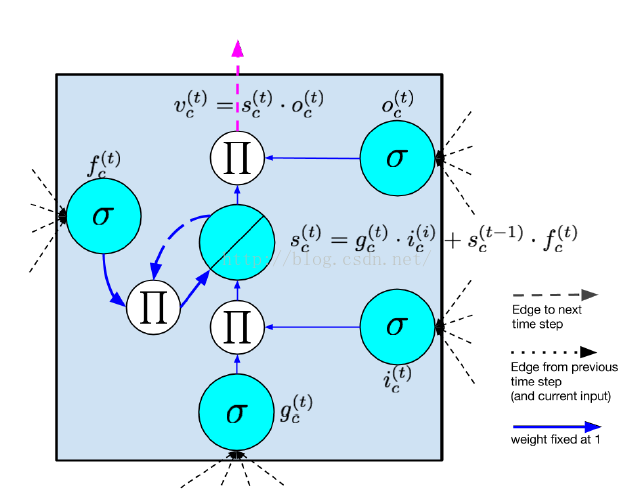
\includegraphics[width=0.6\textwidth]{lstmCell}
	\caption[Một "LSTM cell"]{Mô hình RNN đơn giản với kết nối vòng, \textbf{$h$} được xem như bộ nhớ được luân chuyển trong RNN. Chú ý rằng đường nét đứt ở đầu ra thể hiện rằng tại một thời điểm $t$, RNN có thể có hoặc không có một đầu ra.}
	\label{fig_lstmCell}
\end{figure}

Hochreiter và Schmidhuber \cite{hochreiter1997} đã giới thiệu mô hình \textit{Long short-term memory} (LSTM) chủ yếu ở để khắc phục vấn đề biến mất gradient trong RNN. Nhớ lại rằng trong RNN, chính việc mô hình hóa phụ thuộc thời gian dựa vào ma trận trọng số $W_{hh}$ đã gây ra hiện tượng gradient biến mất. Ý tưởng của LSTM là thay vì tính toán $h_t$ từ $h_{t-1}$ với một phép nhân ma trận theo sau là hàm kích hoạt phi tuyến, LSTM trực tiếp tính toán một $\Delta h_t$ sau đó nó được cộng với $h_{t-1}$ để tạo ra $h_t$. Thoạt nhìn, sự khác biệt này có thể không đáng kể khi mà chúng ta đều đạt được $h_t$ trong cả hai cách. Tuy nhiên, với cách làm này, gradient của $\Delta h_t$ sẽ không bị biến mất.

Thuật ngữ "Long short-term memory" xuất phát từ nhận định sau. Mạng RNN đơn giản có "long term memory" (bộ nhớ dài hạn) dưới dạng các ma trận trọng số. Những ma trận trọng số này thay đổi một cách chậm rãi trong quá trình học nhằm mã hóa kiến thức về dữ liệu. RNN cũng có "short-term memory" (bộ nhớ ngắn hạn) dưới dạng các kích hoạt tạm thời, được truyền từ mỗi bước thời gian sang các bước thời gian sau đó. "Long short-term memory" tạm dịch là "bộ nhớ ngắn hạn dài" cho phép mở rộng bộ nhớ ngắn hạn bằng cách thêm vào một loại lưu trữ trung gian gọi là trạng thái lưu giữ (cell state). Trạng thái lưu giữ này có khả năng lưu giữ các thông tin cần thiết một cách lâu dài dưới dạng một bộ nhớ ngắn hạn. Để làm được điều này, LSTM sử dụng một cơ chế gọi là "cổng", các "cổng" giúp được huấn luyện để chọn lọc thông tin nào là cần thiết để tác động lên trạng thái lưu trữ. Với cách làm này, trạng thái lưu trữ sẽ lưu được nhiều thông tin hơn, vì chỉ những thông tin quan trọng mới tồn tại trong nó.

Về cấu tạo, một LSTM tương tự như một RNN một lớp ẩn, nhưng mỗi "RNN cell" (ký hiệu "A" trong hình \ref{fig_rnn_unrolled}) được thay thế bằng một "memory cell" (hình \ref{fig_lstmCell}). Giống như "RNN cell", "memory cell" nhận một đầu vào bên ngoài và phát sinh một đầu ra cũng như là truyền đi một trạng thái ẩn sang "memory cell" ở bước thời gian kế tiếp. Tuy nhiên, trong "memory cell" còn có thêm một trạng thái lưu giữ cũng được truyền đi như một trạng thái ẩn. Cấu tạo chi tiết của LSTM sẽ được trình bày trong phần dưới đây, cấu tạo này dựa trên phiên bản LSTM của \cite{Gers2000}.

\begin{itemize}
	\item[•] \textit{Nút đầu vào (input node)}: Đơn vị này được ký hiệu là $g$, là một mạng nơ-ron một tầng ẩn. Nút đầu vào có nhiệm vụ mô hình hóa đầu vào tại mỗi bước thời gian. Nó nhận tham số là đầu vào tại bước thời gian hiện tại $x_t$ và trạng thái ẩn tại thời điểm trước đó $h_{t-1}$. Cụ thể, tại mỗi bước thời gian nút đầu vào có công thức:
	\begin{equation} \label{inputNodeLSTM}
		g_t = \phi \left(W_{gx}x_t + W_{gh}h_{t-1} + b_g \right)
	\end{equation}
	\item[•] \textit{Cổng vào (input gate)}: "Cổng" như đã nói, là một cơ chế đặc biệt của LSTM. Cổng vào cũng được cấu tạo giống như nút đầu vào, nó nhận tham số là $x_t$ và $h_{t-1}$. Sau đó được đưa qua hàm kích hoạt $\sigmoid$ để tạo ra giá trị trong khoảng $(0,1)$. Sở dĩ đơn vị này được gọi là "cổng vào" vì giá trị của nó sẽ được sử dụng để nhân với giá trị của nút đầu vào. Giá trị của nó thể hiện lượng thông tin mà nút đầu vào được phép truyền đi. Nếu cổng vào bằng 0, nút đầu vào sẽ truyền đi với giá trị 0. Nếu cổng vào bằng 1, nút đầu vào sẽ truyền đi với giá trị ban đầu. Cụ thể hơn, ta có công thức của cổng vào, được ký hiệu là $i$, tại bước thời gian $t$:
	\begin{equation} \label{inputGateLSTM}
		i_t = \sigma \left(W_{ix}x_t + W_{ih}h_{t-1} + b_i \right)
	\end{equation}
	\item[•] \textit{Trạng thái lưu giữ (cell state)}: Trái tim của LSTM chính là trạng thái lưu trữ, là một mạng nơ-ron với hàm kích hoạt tuyến tính. Khá giống với trạng thái ẩn trong RNN, trạng thái lưu trữ $s_t$ cũng có một kết nối hồi quy với trạng thái lưu trữ trước đó $s_{t-1}$. Tuy nhiên, trọng số kết nối hồi quy luôn có giá trị cố định là 1. Bởi vì kết nối hồi quy này qua nhiều bước đều có trọng số không đổi nên khi tính toán, "gradient" của độ lỗi không bị bùng nổ hay biến mất. Tại mỗi bước thời gian, trạng thái lưu trữ được tính như sau:
	\begin{equation} \label{cellStateLSTM}
		s_t = s_{t-1} + g_t \odot i_t
	\end{equation}
	\item[•] \textit{Cổng quên (forget gate)}: Là trái tim của LSTM. Cổng quên là một đề xuất của \cite{Gers2000} so với bài báo LSTM gốc. Thay vì kiểm soát lượng thông tin để đưa vào trạng thái lưu giữ như cổng vào, cổng quên cung cấp khả năng tẩy đi một lượng thông tin trong trạng thái lưu giữ. Cụ thể, cổng quên với giá trị thuộc khoảng $(0,1)$ sẽ được nhân với $s_{t-1}$ trong công thức \ref{cellStateLSTM}. Tại mỗi bước thời gian, giá trị của cổng quên $f_t$ được tính như sau:
	\begin{equation} \label{forgetGateLSTM}
		f_t = \sigma \left(W_{fx}x_t + W_{fh}h_{t-1} + b_f \right)
	\end{equation}
	Công thức của trạng thái lưu trữ được sửa lại khi có cổng quên:
	\begin{equation} \label{cellStateWithForgetGateLSTM}
		s_t = s_{t-1} \odot f_t + g_t \odot i_t
	\end{equation}
	\item[•] \textit{Cổng ra (output gate)}:
\end{itemize}



\section{Mô hình ngôn ngữ}

Như chúng tôi đã đề cập trong chương 1, \textit{mô hình ngôn ngữ} (language model) là một bộ phận quan trọng trong cả dịch máy thống kê và dịch máy nơ-ron. Cụ thể hơn, mô hình ngôn ngữ là một phân phối xác suất trên một chuỗi các từ. Cho trước một chuỗi $w_1,w_2,...,w_m$ (ký hiệu $w_{1:n}$), mô hình ngôn ngữ gán cho nó một xác suất $P(w_{1:n})$ đại diện cho độ "trơn tru" của chuỗi đó. Sử dụng quy tắc dây chuyền (chain rule) trong xác suất, ta có:
\begin{equation} \label{lmGeneral}
	P(w_{1:n}) = P(w_1)P(w_2|w_1)P(w_3|w_{1:2})P(w_4|w_{1:3})...P(w_n|w_{1:n-1})
\end{equation}















	\chapter{Cơ chế Attention cho mô hình Dịch máy}
\ifpdf
    \graphicspath{{Chapter3/Chapter3Figs/PNG/}{Chapter3/Chapter3Figs/PDF/}{Chapter3/Chapter3Figs/}}
\else
    \graphicspath{{Chapter3/Chapter3Figs/EPS/}{Chapter3/Chapter3Figs/}}
\fi
\label{chap_3}
\begin{quote}
\textit{Chương này trình bày về cơ chế Attention. Ở đây, chúng tôi tập trung tìm hiểu về các phiên bản của cơ chế Attention và đánh giá chúng dựa trên cơ sở Toán học. Cụ thể, chúng tôi tìm hiểu về hai phiên bản Toàn cục (Global) và Cục bộ (Local):
\begin{itemize}
	\item Toàn cục: chúng tôi nhận thấy sự hạn chế hiện có của kiến trúc Bộ mã hóa-Bộ mã hóa khi thực hiện dịch những câu dài. Do vậy, chúng tôi sử dụng cơ chế Attention phiên bản Toàn cục để giải quyết vấn đề này.
	\item Cục bộ: chúng tôi quan sát thấy rằng Attention Toàn cục vẫn còn một chút vấn đề về ý tưởng và chi phí tính toán. Với sự quan sát đó, chúng tôi hiệu chỉnh Attention Toàn cục thành phiên bản Attention Cục bộ để giải quyết những hạn chế đó.
\end{itemize}}
\end{quote}
\section{Cơ chế Attention}
Ở phần trước, chúng tôi đã trình bày về kiến trúc Bộ mã hóa-Bộ giải mã cùng với những điểm mạnh của nó trong việc giải quyết bài toán Dịch máy. Tuy nhiên, kiến trúc này vẫn còn tồn tại hạn chế về việc dịch những câu dài do những thông tin được mã hóa của câu nguồn bị mất dần theo các thời điểm về sau. Lí do mà vấn đề này tồn tại thực chất là bởi vì các mô hình LSTM được sử dụng trong Bộ mã hóa và Bộ giải mã. Bản thân mô hình LSTM chưa thật sự giải quyết hoàn toàn vấn đề "sự phụ thuộc dài hạn". Để có thể vẫn tận dụng được các mô hình LSTM mà vẫn nâng cao được chất lượng dịch, chúng tôi sử dụng cơ chế Attention.

Trước khi đi vào cách hoạt động của cơ chế Attention, chúng tôi điểm qua một chút về nguồn cảm hứng và lịch sử của cơ chế này. Cơ chế Attention được lấy cảm hứng trên cơ chế đặt sự chú ý khi quan sát sự vật, hiện tượng của thị giác con người. Khi con người quan sát một sự vật, hiện tượng nào đó bằng mắt, con người chỉ có thể tập trung vào một vùng nhất định trên sự vật, hiện tượng được quan sát để ghi nhận thông tin. Sau đó, khi cần ghi nhận thêm thông tin khác, con người sẽ di chuyển vùng tập trung lên vật thể của mắt sang vị trí khác. Những vùng lân cận xung quanh vùng tập trung sẽ bị "mờ" hơn so với vùng tập trung. Cơ chế Attention đã được ứng dụng trong lĩnh vực Thị giác máy tính từ khá lâu \cite{attentionhistory2010} \cite{attentionhistory2011}. Vào những năm gần đây, cơ chế Attention được sử dụng cho các kiến trúc mạng nơ-ron hồi quy trên bài toán Dịch máy và đã đạt được những kết quả ấn tượng.

\begin{figure}
	\centering
	\includegraphics[width=0.8\textwidth]{Attention-2}
	\caption[Minh họa cơ chế Attention.]{Minh họa cơ chế Attention. Một tầng Attention được đặt ở trước bước dự đoán đầu ra của bộ giải mã.}
	\label{fig_Attention}
\end{figure}
Cơ chế Attention được sử dụng trong đề tài này là một cơ chế sử dụng thông tin trong các trạng thái ẩn của RNN trong bộ mã hóa khi thực hiện quá trình giải mã. Cụ thể là:
\begin{itemize}
	\item Trong quá trình giải mã, trước khi dự đoán đầu ra, bộ giải mã nhìn vào các thông tin nằm trong các trạng thái ẩn của RNN ở bộ mã hóa.
	\item Ở mỗi phần tử đầu ra tại thời điểm $t$, bộ giải mã dựa vào trạng thái ẩn tại thời điểm $t$ hiện tại và quyết định sử dụng các thông tin trong trạng thái ẩn ở bộ mã hóa như thế nào.
\end{itemize}
2 phiên bản Toàn cục và Cục bộ mà trong khóa luận này chúng tôi trình bày là 2 cách mà cơ chế Attention sử dụng các trạng thái ẩn của RNN trong bộ mã hóa.
Để làm rõ hơn về ý tưởng của cơ chế Attention, dưới đây chúng tôi sẽ trình bày chi tiết về nền tảng Toán học của nó.
Attention sử dụng thêm một số đại lượng:
\begin{itemize}
	\item $a_t$: trọng số gióng hàng, $a_t$ được tính theo công thức dưới đây:
	\begin{equation}
	a_t = \text{align}(h_t, \bar{h}_s) = \frac{\exp\left(\text{score}(h_t, \bar{h}_s)\right)}{\sum_{s^{'}}\exp\left(\text{score}(h_t, \bar{h}_{s^{'}})\right)}
	\end{equation}
	$a_t$ là một véc-tơ chứa các điểm số giữa trạng thái ẩn ở thời điểm $t$ $h_t$ và các trạng thái ẩn ở câu nguồn $\bar{h}_s$. Hàm điểm số score mà chúng tôi sử dụng là gồm 2 hàm:
	\begin{equation}
	\text{score}(h_t, \bar{h}_s) = \left\{
			\begin{array}{ll}
			h^T_t\bar{h}_s \ \quad\quad dot\\
			h^T_tW_a\bar{h}_s	\quad general
			\end{array}
		\right.
	\end{equation}
	Đối với hàm score là hàm \textit{dot}, mô hình chỉ đơn giản là thực hiện tính độ tương đồng giữa 2 trạng thái ẩn. Giá trị của hàm score đạt cao nhất khi 2 véc-tơ trạng thái ẩn hoàn toàn giống nhau. Ưu điểm của hàng \textit{dot} này là chi phí tính toán thấp nên thời gian huấn luyện và suy diễn nhanh.
	Đối với hàm score là hàm \textit{general}, hàm này có sự tinh tế hơn hàm \textit{dot}. Hàm \textit{dot} thực hiện tính sự tương đồng lên tất cả cặp phần tử trong 2 véc-tơ, trong khi đó hàm \textit{general} sử dụng thêm một bộ trọng số $W_a$, do đó những thông tin giữa hai trạng thái ẩn sẽ được tính một cách chọn lọc hơn. Tuy nhiên, đổi lại thì hàm này sẽ có thời gian thực thi chậm hơn hàm \textit{dot} một chút. Trong thực tế, không có minh chứng rõ ràng nào cho thấy rằng hàm nào sẽ tốt hơn, do vậy cần phải thực nghiệm cẩn thận để có được sự lựa chọn chính xác nhất.
	\item $c_t$: véc-tơ ngữ cảnh tại thời điểm $t$, là trung bình có trọng số của các trạng thái ẩn ở câu nguồn:
	\begin{equation}
	c_t = \sum_{s}a_{ts}h_s
	\end{equation}
	Véc-tơ $c_t$ cho mô hình biết thông tin rằng với trạng thái ẩn hiện tại (chứa thông tin của quá trình dịch trước đó) thì ngữ cảnh hiện của thời điểm $t$ hiện tại là gì. Ngữ cảnh đó được thể hiện thông qua những thông tin của các trạng thái ẩn $h_s$ của câu nguồn mà được lựa chọn một cách có chọn lọc (có trọng số). Véc-tơ ngữ cảnh $c_t$ là một cách biểu diễn ngữ cảnh của ngôn ngữ đích bằng ngữ cảnh của ngôn ngữ nguồn. Trong quá trình dịch, bộ giải mã cần phải dự đoán từ tiếp theo của câu dịch. Để dự đoán được chính xác, mô hình cần phải biết được ngữ cảnh hiện tại của câu là gì. Để đảm bảo ngữ cảnh mà mô hình nhận được chính xác, mô hình không thể chỉ dựa vào các trạng thái ẩn của bộ giải mã ở các thời điểm trước đó. Do vậy, mô hình sử dụng thêm các trạng thái ẩn của các từ ở câu nguồn để thể hiện ngữ cảnh một cách chính xác hơn.
	\item $\tilde{h}_t$, véc-tơ attention tại thời điểm $t$, được tính như sau:
	\begin{equation}
	\boldsymbol{\tilde{h}_t} = \tanh(\bm{W_c}[\bm{c_t};\bm{h_t}])
	\end{equation}
	Véc-tơ attention chứa thông tin gióng hàng và trạng thái ẩn của thời điểm $t$ hiện tại. Nhờ đó, mô hình nắm giữ được nhiều thông tin hơn để có thể dự đoán tốt hơn.
\end{itemize}
Bước dự đoán đầu ra không thay đổi ngoài trạng thái ẩn $\bm{h_t}$ được thay thế bởi véc-tơ attention $\bm{\tilde{h}_t}$. $\bm{\tilde{h}_t}$ được đưa qua tầng softmax để cho ra phân bố xác suất dự đoán trên các từ:
\begin{equation}
p(y_t | y_{<t}, x) = \text{softmax}(\bm{W_s\tilde{h}})
\end{equation}
Nói một cách đơn giản, mục tiêu của cơ chế Attention là xoay quanh việc tìm véc-tơ ngữ cảnh $c_t$ một cách hiệu quả.
Tiếp theo, chúng tôi trình bày chi tiết hơn về 2 phiên bản Toàn cục và Cục bộ. 2 phiên bản này chỉ khác nhau về cách suy ra véc-tơ ngữ cảnh $\bm{c_t}$, còn các bước còn lại giống nhau.
Quy trình tính toán của cơ chế Attention: $h_t -> a_t -> c_t -> \tilde{h}_t$
\section{Attention Toàn cục}
Ý tưởng của Attention toàn cục là nhìn vào toàn bộ các vị trí nguồn (các trạng thái ẩn của RNN ở bộ mã hóa) khi thực hiện giải mã.
Khi đó trọng số gióng hàng $a_t$ là một véc-tơ có kích thước thay đổi và bằng số trạng thái ẩn (số từ) ở câu nguồn: $\text{len}(a_t) = S$.

\begin{equation}
a_t = \text{align}(h_t, \bar{h}_s) = \frac{\exp\left(\text{score}(h_t, \bar{h}_s)\right)}{\sum^{S}_{s^{'}=1}\exp\left(\text{score}(h_t, \bar{h}_{s^{'}})\right)}
\end{equation}

\begin{figure}
	\centering
	\includegraphics[width=0.8\textwidth]{Global-Attention_2.png}
	\caption[Minh họa cơ chế Attention Toàn cục.]{Minh họa cơ chế Attention Toàn cục. Tại thời điểm $t$, bộ giải mã nhìn vào toàn bộ trạng thái ẩn ở các vị trí nguồn.}
	\label{fig_Global_Attention}
\end{figure}

Ưu điểm của phương pháp này là ý tưởng đơn giản, dễ cài đặt nhưng vẫn đạt được hiệu quả tốt (sẽ được trình bày ở phần thực nghiệm). Tuy nhiên, ý tưởng này vẫn còn chưa thực sự tự nhiên và còn hạn chế. Khi dịch một từ thì không cần phải đặt "sự chú ý" lên toàn bộ câu nguồn, chỉ cần đặt "sự chú ý" lên một số từ cần thiết. Mặc dù khi mô hình Attention Toàn cục được huấn luyện tốt thì hoàn toàn có thể chỉ đặt "sự chú ý" lên một số từ thật sự cần thiết, nhưng dễ thấy rằng bản thân mô hình vẫn phải tiêu tốn chi phí cho việc tính toán trọng số gióng hàng $a_t$ cho những vị trí không cần thiết. Đó là trường hợp lý tưởng cho mô hình Attention Toàn cục, nhưng trong thực tế, để đạt được độ chính xác như thế thì phải tiêu tốn nhiều tài nguyên cho việc huấn luyện mô hình như tài nguyên về tập dữ liệu đủ lớn, đủ tốt hay thời gian huấn luyện phải đủ lâu.
Để giải quyết hạn chế trên của Attention Toàn cục, chúng tôi đã tìm hiểu và sử dụng phiên bản tinh tế hơn, đó là mô hình Attention Cục bộ. Ở phần tiếp theo, chúng tôi sẽ trình bày về mô hình này.

\section{Attention Cục bộ}
Như đã nêu ở phần trước, Attention Toàn cục có một hạn chế là đặt "sự chú ý" lên toàn bộ các từ ở câu nguồn khi dịch từng từ ở câu đích. Điều này gây tiêu tốn chi phí tính toán và có thể tạo ra những câu dịch không thực tế khi dịch những câu dài như trong các đoạn văn hay trong một tài liệu. Attention Cục bộ ra đời để giải quyết hạn chế này.

Khi dịch mỗi từ ở câu đích, Attention Cục bộ chỉ đặt "sự chú ý" lên một số từ gần nhau ở câu nguồn. Mô hình này lấy cảm hứng từ sự đánh đổi giữa 2 mô hình "soft attention" và "hard attention" được đề xuất trong công trình Show, Attend and Tell \cite{showattendandtellXu2015} để giải quyết bài toán Phát sinh câu miêu tả cho ảnh (Image Captioning). Trong công trình \cite{showattendandtellXu2015}, Attention Toàn cục tương ứng với "soft attention", "sự chú ý" được đặt trên toàn bộ bức ảnh. Còn "hard attention" thì đặt "sự chú ý" lên một số phần của bức ảnh.

Dễ thấy, với cách hoạt động chỉ tập trung một số các từ gần nhau ở câu nguồn, mô hình hoạt động gần với cách con người tập trung vào một sự vật, hiện tượng nào đó. Chi phí cho huấn luyện và dự đoán sẽ được giảm bớt bởi vì chúng ta chỉ thực hiện tính véc-tơ trọng số gióng hàng $a_t$ cho những từ mà mô hình đặt "sự chú ý" lên.

Để làm rõ hơn về cách thức hoạt động của mô hình Attention Cục bộ, chúng tôi sẽ trình bày cụ thể hơn về nền tảng Toán học của mô hình này. Bên cạnh những đại lượng đã có ở mô hình Attention Toàn cục, Attention Cục bộ có thêm và thay đổi một số đại lượng như sau:
\begin{itemize}
	\item $p_t$: vị trí đã được gióng hàng. Tại mỗi thời điểm $t$, mô hình sẽ phát sinh một số thực $p_t$. Số thực này có giá trị nằm trong đoạn $[0, S]$ với ý nghĩa rằng đây là vị trí đã được gióng hàng của với từ ở câu nguồn tại thời điểm $t$ hiện tại. Hay nói cách khác, "sự chú ý" được đặt trên từ có vị trí $p_t$ này. Để ý thấy rằng có sự không tự nhiên khi $p_t$ là một số thực, do vậy $p_t$ không thể cho biết được chính xác từ nào sẽ được đặt "sự chú ý" lên. Thực tế, với miền giá trị số thực, $p_t$ có tác dụng là dùng để làm vị trí trung tâm cho các từ lân cận. Để làm rõ hơn về vấn đề này, chúng tôi sẽ trình bày rõ ràng hơn ở sau.
	\item Đối quá trình tính véc-tơ ngữ cảnh $c_t$ có sự thay đổi rằng mô hình xét các vị trí ở câu nguồn mà nằm xung quanh vị trí $p_t$ một đoạn $D$. $D$ là một đại lượng với miền số nguyên lớn hơn 0 và được gọi là kích thước cửa sổ. Cụ thể:
	\begin{equation}
	c_t = \sum_{x \in [p_t - D, p_t + D]} a_{tx}\tilde{h}_x
	\end{equation}
	$D$ là một siêu tham số của mô hình. Việc lựa chọn giá trị của $D$ là dựa vào thực nghiệm. Theo đề xuất của \cite{attentionThangLuong2015}, chúng tôi lựa chọn $D = 10$.
\end{itemize}

\begin{figure}
	\centering
	\includegraphics[width=0.8\textwidth]{Local-Attention_2.png}
	\caption[Minh họa cơ chế Attention Cục bộ.]{Minh họa cơ chế Attention Cục bộ. Tại thời điểm $t$, bộ giải mã nhìn vào một số trạng thái ẩn ở các vị trí nguồn.}
	\label{fig_Local_Attention}
\end{figure}

Mô hình Attention Cục bộ có 2 biến thể:
\begin{itemize}
	\item Gióng hàng đều (monotonic alignment - local-m): vị trí được gióng hàng được phát sinh một cách đơn giản bằng cách cho $p_t = t$ tại mỗi thời điểm $t$. Ta giả định rằng các từ ở câu nguồn và các từ ở câu đích được gióng hàng đều nhau theo từng từ.
	\item Gióng hàng dự đoán (predictive alignment - local-p): giả định rằng tất cả từ ở câu nguồn và câu đích đều được gióng hàng đều nhau không thực tế vì giữa 2 ngôn ngữ có ngữ pháp riêng và trật tự từ khác nhau. Chúng tôi sẽ trình bày rõ ràng hơn vào các phần sau. Do vậy, mô hình sẽ phát sinh vị trí được gióng hàng $p_t$ một cách tự nhiên hơn cho phù hợp đặc điểm của ngôn ngữ. Cụ thể mô hình sẽ phát sinh vị trí $p_t$ tại mỗi thời điểm $t$ như sau:
	\begin{equation}
	p_t = S \cdot \text{sigmoid} (v^T_p \tanh(W_p h_t))
	\end{equation}
	Trong đó, $v_p$ và $W_p$ là 2 tham số mới của mô hình cho việc dự đoán vị trí $p_t$. Mô hình cần học 2 tham số này. Miền giá trị của $p_t \in [0, S]$.
	Để "ưu tiên" các vị trí được gióng hàng $p_t$, mô hình thêm vào trọng số gióng hàng của những từ lân cận đó một lượng có giá trị bằng giá trị của phân phối chuẩn (Gauss) mà đã được đơn giản hóa với trung bình $p_t$ và độ lệch chuẩn $\sigma = \frac{D}{2}$:
	\begin{equation}
	p_t = \text{align}(h_t, \bar{h}_s)\exp\left(-\frac{(s-p_t)^2}{2\sigma^2}\right)
	\end{equation}
	Mô hình sử dụng hàm gióng hàng như các phiên bản trước. $s$ là giá trị số nguyên thể hiện các vị trí nằm xung quanh $p_t$ mà nằm trong cửa sổ $D$.
\end{itemize}
 Đối với những vị trí $s$ nằm ngoài câu (cửa sổ $D$ vượt qua các biên của câu) thì mô hình sẽ bỏ qua những vị trí $s$ nằm ngoài và chỉ xem xét những vị trí $s$ nằm trong biên của câu.
 
 Véc-tơ trọng số gióng hàng $a_t$ ở Attention Cục bộ có kích thước cố định $\in \mathbb{R}^{2D + 1}$ và thường ngắn hơn $a_t$ ở Attention Toàn cục. Local-p và local-m giống nhau chỉ khác rằng local-p tính vị trí $p_t$ một cách linh hoạt và sử dụng một phân phối chuẩn đã được đơn giản hóa để điều chỉnh các trọng số gióng hàng gốc $\text{align}(h_t, \bar{h}_s)$. Việc sử dụng thêm phân phối chuẩn để khuyến khích mô hình đặt "sự chú ý" lên vị trí $p_t$ và phân chia dần cho các vị trí lân cận. Nếu không có việc sử dụng phân phối chuẩn này, mô hình có thể sẽ đặt "sự chú ý" hoàn toàn lên các từ lân cận xung quanh $p_t$ mà không phải là vị trí $p_t$. Điều này không phù hợp với ý tưởng ban đầu của việc phát sinh vị trí $p_t$.
Với cơ chế được trình bày cụ thể như trên, mô hình Attention Cục bộ hoạt động tự nhiên hơn, phù hợp với cách con người đặt "sự chú ý" khi quan sát sự vật, hiện tượng. Bên cạnh đó, Attention Cục bộ giảm chi phí tính toán của mô hình.

\section{Phương pháp Input feeding}
Trong quá trình dịch, các mô hình được đề cập ở trên như Attention Toàn cục hay Cục bộ, đều vẫn còn một hạn chế về cách đặt "sự chú ý" hay gióng hàng lên các vị trí nguồn. Ở mỗi thời điểm $t$ khi dịch một từ ở câu đích, việc đặt "sự chú ý" của thời điểm $t$ độc lập hoàn toàn với việc đặt "sự chú ý" ở các thời điểm trước đó. Việc quyết định gióng hàng như thế nào (véc-tơ $a_t$) hoàn toàn phụ thuộc vào điểm số (giá trị của hàm score) giữa trạng thái ẩn $h_t$ hiện tại và các trạng thái ẩn $\bar{h}_s$ ở câu nguồn. Trong thực tế, khi dịch, một từ ở câu nguồn chỉ tương ứng với một vài từ ở câu đích. Do vậy, mô hình cần phải theo dõi xem là những từ nào ở câu nguồn đã được dịch trước đó thì hạn chế đặt "sự chú ý" lên lại những từ đó. Việc không có cơ chế kiểm soát những từ nào đã được dịch sẽ khiến cho mô hình sẽ rơi vào 2 trường hợp "được dịch quá nhiều" (over-translated) hoặc "được dịch quá ít" (under-translated). Tức là có một số từ ở câu nguồn sẽ được đặt "sự chú ý" lên quá nhiều lần dẫn tới bỏ qua những từ quan trọng khác hoặc là một số từ quan trọng được đặt "sự chú ý" lên quá ít dẫn tới việc bỏ qua thông tin của từ đó trong quá trình dịch. Dù là trường hợp nào thì cũng gây giảm chất lượng dịch của mô hình.

Trong Dịch máy Thống kê, Koehn et al. 2003 \cite{smtKoehn2003} đã đề xuất một mô hình dịch dựa trên cụm từ (phrase-based) mà có cơ chế để giải quyết vấn đề trên. Cơ chế này rất đơn giản và trực quan. Trong quá trình dịch, bộ giải mã duy trì một véc-tơ bao phủ (coverage vector) để chỉ ra rằng từ ở câu nguồn nào đã được dịch hoặc chưa được dịch. Quá trình dịch được hoàn thành khi toàn bộ từ ở câu nguồn được "bao phủ" hay dẵ được dịch. Trong khi đó, các mô hình Dịch máy Nơ-ron hiện nay chỉ kết thúc quá trình dịch khi và chỉ khi gặp kí tự kết thúc câu hoặc vượt quá số lượng từ cho trước. Việc này dễ dẫn đến trường hợp "được dịch quá nhiều" khi kí hiệu kết thúc câu xuất hiện trễ hay ngược lại dẫn đến trường hợp "được dịch quá ít" khi kí hiệu kết thúc câu xuất hiện sớm. Ngoài ra còn bị ảnh hưởng bởi số lượng từ quy định khi dịch.

Công trình \cite{attentionThangLuong2015} đề xuất một cơ chế góp phần giải quyết vấn đề ở trên:  (tạm dịch là "cho đầu vào ăn" // TODO: dịch khác). Ý tưởng và cách thực hiện của Input feeding rất đơn giản. Nhận thấy véc-tơ attention $\tilde{h}_{t-1}$ lưu giữ thông tin gióng hàng của thời điểm $t-1$ trước đó, mô hình thực hiện truyền véc-tơ $\tilde{h}_{t-1}$ vào đầu vào $x_t$ của thời điểm $t$ hiện tại. Bằng cách như vậy, mô hình có thể nắm được thông tin gióng hàng trước đó từ $\tilde{h}_{t-1}$. Cụ thể, véc-tơ $\tilde{h}_{t-1}$ được nối với véc-tơ đầu vào của thời điểm $t$ là $x_t$:
\begin{equation}
x^{'}_t = [x_t, \tilde{h}_t]
\end{equation}

\begin{figure}
	\centering
	\includegraphics[width=0.8\textwidth]{Input-feeding_2.png}
	\caption[Minh họa cơ chế Attention Cục bộ.]{Minh họa phương pháp Input feeding. Tại thời điểm $t$, bộ giải mã nhận đầu vào gồm véc-tơ attention ở thời điểm trước đó $t-1$ và từ hiện tại $x_t$.}
	\label{fig_Input_feeding}
\end{figure}
Tuy nhiên, phương pháp này chưa thực sự giải quyết triệt để vấn đề "được dịch quá nhiều" hay "được dịch quá ít". Vì mô hình chỉ nhận được thông tin gióng hàng từ các thời điểm trước đó nhưng lại không được hướng dẫn, ràng buộc cụ thể nào mà có thể giải quyết vấn đề này. Việc giải quyết vấn đề trên hoàn toàn phụ thuộc vào quyết định của mô hình . Mặc dù chưa thực sự giải quyết triệt để, nhưng lại cho mô hình tăng thêm tính mềm dẻo trong việc sử dụng thông tin gióng hảng trước đó. Trong thực tế, phương pháp này đã cải thiện chất lượng dịch lên đáng kể.

Ngoài ra, phương pháp này giúp cho mô hình phức tạp hơn nhờ vào việc đưa véc-tơ attention $\tilde{h}_{t}$ vào đầu vào của thời điểm tiếp theo, đồng thời làm tăng khả năng học của mô hình.

\section{Kĩ thuật thay thế từ hiếm}
Trong quá trình dịch thuật, có rất nhiều hạn chế gây ảnh hưởng tới chất lượng của bản dịch. Trong phần này, chúng tôi đề cập tới một vấn đề quan trọng mà dù là con người hay máy tính đều gặp phải và rất khó giải quyết. Đó là vấn đề về những "từ hiếm" (unknown words). 

Mỗi ngôn ngữ có muôn hình vạn trạng các từ ngữ khác nhau. Số lượng từ ngữ trong một ngôn ngữ là không có định. Trong quá trình hình thành và phát triển ngôn ngữ, theo thời gian số lượng từ ngữ sẽ tăng lên hoặc mất đi (bị lãng quên hay không dùng nữa) tùy thuộc vào hoàn cảnh, môi trường sử dụng của ngôn ngữ đó. Nhưng thường đối với những ngôn ngữ phổ biển hiện nay thì số lượng từ ngữ tăng lên lớn hơn nhiều so với số lượng từ ngữ mất đi. Khi xã hội phát triển, nhu cầu giao tiếp giữa các dân tộc, quốc gia, nền văn hóa khác nhau cũng tăng theo. Mỗi nơi lại có cách sử dụng ngôn ngữ khác nhau, do đó bộ từ vựng của mỗi ngôn ngữ cũng phải thay đổi sao cho phù hợp với nhu cầu giao tiếp. Khoa học kĩ thuật phát triển kèm theo đó là những khám phá về thế giới tự nhiên. Những sự vật, hiện tượng mới được phát hiện ngày càng nhiều. Và không phải sự vật, hiện tượng nào cũng có thể được mô tả, thể hiện bằng những vốn từ vựng vốn có của một số ngôn ngữ. Ngoài ra còn có nhiều lí do làm cho bộ từ vựng của các ngôn ngữ thay đổi theo thời gian.

Với tốc độ phát triển của ngôn ngữ là như vậy nhưng khả năng của con người là hữu hạn. Một người dù có thông thạo một ngôn ngữ tới đâu thì cũng không thể nào biết được hết tất cả từ vựng của ngôn ngữ đó. Theo thống kê, số lượng từ ngữ cần để giao tiếp hàng ngày trong tiếng Anh chỉ khoảng từ 2000-3000 từ, đối với lĩnh vực chuyên ngành thì khoảng 5000-6000 từ. Nhưng theo kích thước của một số bộ từ điển thịnh hành trong tiếng Anh thì số lượng từ vựng của những bộ từ điển đó khoảng 60000 từ. Tức là đa số mọi người chưa biết hết được 10\% từ vựng của tiếng Anh. Do vậy khi thực hiện việc dịch thuật giữa các ngôn ngữ với nhau, mọi người chỉ có thể dịch tốt khi văn bản, hội thoại cần dịch thuộc về chủ đề mà họ quen thuộc. Mọi người sẽ gặp khó khăn khi gặp những từ nằm ngoài bộ từ vựng của bản thân (out-of-vocabulary words - OOV words) vì không biết phải dịch như thế nào.

Khi huấn luyện một mô hình Dịch máy thì cần phải có một bộ từ vựng cố định cho mô hình đó trong suốt quá trình huấn luyện và dự đoán. Kích thước của bộ từ vựng này bị hạn chế với số lượng nhất định. Sự hạn chế về kích thước này xuất phát từ nhiều lí do như giới hạn về dữ liệu huấn luyện, khả năng học của mô hình, tài nguyên tính toán (phần cứng), v.v... Do vậy việc quyết định xem những từ nào sẽ được đưa vào bộ từ vựng của mô hình cũng rất quan trọng. Thông thường có 2 chiến thuật để xây dựng bộ từ vựng này. Cách đầu tiên phù hợp cho việc phát triển các ứng dụng là lấy các từ vựng có trong dữ liệu huấn luyện làm bộ từ vựng và lọc ra những từ nào có tần số xuất hiện trong dữ liệu huấn luyện thấp hơn một ngưỡng nhất định (ví dụ: lọc ra những từ vựng nào có tần số xuất hiện ít hơn 10). Cách thứ 2 thường phù hợp cho việc nghiên cứu, đó là lựa chọn số lượng từ vựng nhất định mà có tần số xuất hiện cao nhất (ví dụ: lấy 50000 từ có tần số xuất hiện cao nhất). Do đó có những từ xuất hiện trong dữ liệu huấn luyện nhưng vì có tần số xuất hiện thấp nên bị coi là từ nằm ngoài bộ từ vựng (OOV). Đó là lí do chúng tôi gọi đây là vấn đề "từ hiếm".

Có nhiều cách để giải quyết vấn đề này, cách mà mọi người hay sử dụng nhất là thêm từ mới đó vào bộ từ vựng. Cách thứ 2 là giữ nguyên từ đó và đưa nó vào vị trí thích hợp trong câu ở ngôn ngữ đích. Trong khóa luận này chúng tôi sẽ sử dụng cách thứ 2 để giải quyết vấn đề các từ nằm ngoái bộ từ vựng.

Kĩ thuật thay thế từ hiếm mà chúng tôi trình bày sau đây là một phương pháp dựa trên kết quả của cơ chế Attention. Do vậy, hiệu quả của phương pháp này phụ thuộc lớn vào độ chính xác của cơ chế Attention. Kĩ thuật này chúng tôi sử dụng từ bài báo của Jean et al., 2015 \cite{JeanUnkRepl} về sử dụng cơ chế Attention trong mô hình Dịch máy nơ-ron. Nếu mô hình không sử dụng cơ chế Attention thì cũng không sử dụng được phương pháp thay thế từ hiếm này. Kĩ thuật này chỉ được sử dụng trong quá trình dự đoán, trong quá trình huấn luyện thì không sử dụng. Cách hoạt động của phương pháp này rất đơn giản. Sau khi mô hình đã dự đoán (dịch) xong một câu, mô hình sẽ thực hiện xử lý những từ nào mà được dự đoán là từ hiếm (unknown words) trong câu đã được dự đoán (những từ hiếm được ký hiệu là \textit{<unk>}). Đối với mỗi từ hiếm, mô hình sẽ thực hiện dịch lại từ đó bằng cách chọn một từ phù hợp trong câu nguồn rồi thực hiện sao chép từ được chọn vào từ hiếm hiện tại. Cách mà mô hình lựa chọn từ phù hợp là dựa vào véc-tơ trọng số gióng hàng $a_t$. Mô hình sẽ lựa chọn từ nào có trọng số cao nhất.

\begin{figure}
	\centering
	\includegraphics[width=0.5\textwidth]{unk-rpl-example.png}
	\caption[Minh họa kĩ thuật thay thế từ hiếm.]{Minh họa phương pháp thay thế từ hiếm. Khi gặp một từ hiếm (được kí hiệu là <unk>) trong kết quả dự đoán, mô hình sẽ tìm một từ ở câu nguồn có trọng số gióng hàng từ kết quả cơ chế Attention cao nhất và thực hiện sao chép từ đó thay cho từ hiếm hiện tại. (Mũi tên càng đậm thì trọng số gióng hàng càng cao). Kết quả dự đoán được cập nhật với từ hiếm đã được thay thế. }
	\label{fig_unk_rpl_example}
\end{figure}

Với kĩ thuật đơn giản là tận dụng ý nghĩa của kết quả của cơ chế Attention, kĩ thuật này đã cải thiện kết quả dịch lên một cách rõ rệt (sẽ được trình bày ở trong phần thực nghiệm).



	\chapter{Các Kết Quả Thực Nghiệm}
\ifpdf
    \graphicspath{{Chapter4/Chapter4Figs/PNG/}{Chapter4/Chapter4Figs/PDF/}{Chapter4/Chapter4Figs/}}
\else
    \graphicspath{{Chapter4/Chapter4Figs/EPS/}{Chapter4/Chapter4Figs/}}
\fi
\label{chap_4}
\begin{quote}
\textit{Trong chương này, chúng tôi trình bày các kết quả thí nghiệm để đánh giá các mô hình được tìm hiểu mà đã trình bày ở chương trước. Bộ dữ liệu được dùng để tiến hành các thí nghiệm là bộ WMT'14 English-German (bộ dữ liệu tiếng Anh-tiếng Đức của cuộc thi Dịch máy WMT năm 2014). Các kết quả thí nghiệm cho thấy khi huấn luyện mô hình mà không sử dụng cơ chế Attention thì kết quả đạt được rất thấp. Các kết quả cũng cho thấy rằng các mô hình Attention Toàn cục, Attention Cục bộ, phương pháp Input feeding cho kết quả được cải thiện một cách rõ rệt.}
\end{quote}
\section{Các thiết lập thực nghiệm}
Chúng tôi tiến hành các thực nghiệm trên bộ dữ liệu WMT' 14 English-German được cung cấp trên trang chủ của Nhóm Xử lý Ngôn ngữ Tự nhiên Đại học Stanford \cite{StanfordNMT}. Bộ dữ liệu này gồm các cặp câu được viết dưới dạng ngôn ngữ tự nhiên ở 2 ngôn ngữ là tiếng Anh và tiếng Đức. Tất cả mô hình sẽ được huấn luyện trên tập dữ liệu này. Tập dữ liệu có khoảng 4,5 triệu cặp câu (trong đó có khoảng 116 triệu từ tiếng Anh và khoảng 110 triệu từ tiếng Đức). Chúng tôi thực hiện thiết lập thực nghiệm giống với các thiết lập của bài báo của Luong et al., 2015 \cite{attentionThangLuong2015}.

Dữ liệu được tiến hành tiền xử lý bằng cách thực hiện tách từ đối với mỗi câu. Bộ từ vựng cho mỗi ngôn ngữ được sử dụng cho các mô hình là bộ từ vựng có 50.000 từ xuất hiện nhiều nhất (có tần số lớn nhất) trong dữ liệu huấn luyện của mỗi ngôn ngữ đó. Những từ nào không nằm trong bộ từ vựng sẽ được gán cho kí hiệu $<unk>$.

Trong quá trình huấn luyện, chúng tôi lọc bỏ những cặp câu mà một trong 2 câu thuộc cặp đó có chiều dài hơn 50 từ. Chúng tôi thực hiện sắp xếp tất cả câu theo chiều dài của câu giảm dần (những câu nào có chiều dài lớn nhất thì đứng đầu), sau đó lấy ngẫu nhiên các mini-batches từ những câu đã được sắp xếp. Với việc sắp xếp như vậy, tốc độ huấn luyện của mô hình được cải thiện và mô hình học được tốt hơn.

Chúng tôi sử dụng các mô hình LSTM với mỗi LSTM có 4 tầng. Mỗi tầng LSTM có kích thước trạng thái ẩn là 1000 (sử dụng Bi-LSTM nên mỗi chiều sẽ có kích thước trạng thái ẩn là 500) và số chiều của word embedding là 1000. Các tham số của mô hình được khởi tạo ngẫu nhiên với phân phối đều trong đoạn $[-0,1; 0,1]$. Thuật toán để cực tiểu hóa hàm chi phí là Stochastic Gradient Descent (SGD) với kích thước của mini-batch là 128 mẫu huấn luyện. Cách lập lịch cho hệ số học: huấn luyện 12 epochs; hệ số học ban đầu là 1,0; sau 8 epochs, hệ số học sẽ giảm đi 1 nửa sau mỗi epoch tiếp theo. Gradient của các tham số sẽ được chuẩn hóa nếu norm của chúng vượt quá 5,0. Mô hình còn sử dụng cơ chế Dropout với xác suất tắt các nơ-ron $p = 0.2$. Mỗi câu ở ngôn ngữ nguồn khi được đưa vào mô hình thì sẽ được đảo ngược trật tự. Đối với các mô hình Attention Cục bộ, kích thước cửa sổ $D = 10$.

Chúng tôi sử dụng ngôn ngữ lập trình Python và framework PyTorch dành cho Học sâu \cite{pytorchworkshop}. PyTorch hỗ trợ việc cài đặt các thuật toán một cách thân thiện, tự nhiên giống như Python và còn hỗ trợ xử lí tính toán song song trên GPU (Graphical Processing Units) rất mạnh mẽ. GPU mà chúng tôi sử dụng để thực hiện các thực nghiệm là NVIDIA GeForce GTX 1080 Ti. Để có thể huấn luyện một mô hình, cần đến 3-5 ngày.

Để đánh giá chất lượng dịch của các mô hình đã được huấn luyện, chúng tôi sử dụng tập dữ liệu kiểm thử \textit{newstest\_2014.en} và \textit{newstest\_2014.de} của cuộc thi WMT'14 và độ đo được sử dụng để đành giá là BLEU (BiLingual Evaluation Understudy) \cite{BLEUpaper} cùng với Perplexity. Dữ liệu validation được sử dụng là tập dữ liệu kiểm thử \textit{newstest\_2013.en} và \textit{newstest\_2013.de} của cuộc thi WMT'13.

Để đánh giá độ hiệu quả của cơ chế Attention , chúng tôi tiến huấn luyện một mô hình cơ bản (Baseline) mà không sử dụng cơ chế Attention (chỉ dùng kiến trúc Bộ mã hóa-Bộ giải mã với các LSTM). Các mô hình có sử dụng cơ chế Attention sẽ được so sánh với mô hình cơ bản này.

\section{Kết quả thực nghiệm}
Các kết quả của các mô hình được ghi trong bảng \ref{wmt14-results}:

\subsection{Không sử dụng Attention và có sử dụng Attention}
Chúng tôi thực hiện đánh giá độ hiệu quả của cơ chế Attention bằng cách so sánh với mô hình không sử dụng cơ chế Attention và các mô hình có sử dụng cơ chế Attention.

Đối với mô hình không sử dụng cơ chế Attention, chúng tôi sử dụng: 
\begin{itemize}
	\item Kiến trúc Bộ mã hóa-Bộ giải mã với bộ mã hóa là bi-LSTM và bộ giải mã là uni-LSTM.
	\item Đảo ngược trật tự từ trong câu.
	\item Dropout.
\end{itemize}
Chúng tôi gọi đó là mô hình cơ bản. Đối với mô hình sử dụng cơ chế Attention, chúng tôi thiết lập mô hình như mô hình căn bản cộng với sử dụng cơ chế Attention Toàn cục với hàm tính điểm là hàm \textit{dot}.

Bảng \ref{tab_non-attn_vs_attn} cho thấy kết quả giữa 2 mô hình. Với cơ chế Attention, chất lượng dịch của mô hình được cải thiện rất lớn. Điểm BLEU tăng từ 15.04 đến 19.02 (+3.98). Đây là bước tiến lớn trong Dịch máy nơ-ron khi Dịch máy Thống kê đang dần chạm tới giới hạn. Kết quả này chứng minh được rằng cơ chế Attention rất hiệu quả trong việc giải quyết các hạn chế của kiến trúc Bộ mã hóa-Bộ giải mã với LSTM ban đầu và cũng rất phù hợp với bài toán Dịch máy.

\begin{table}
	\centering
	\begin{tabular}{|l|l|c|} 
		\hline
		\multicolumn{1}{|c|}{\textbf{Mô hình}} & \textbf{Perplexity} & \textbf{BLEU}  \\ 
		\hline
		Cơ bản                                 &                     & 15.04          \\ 
		\hline
		Cơ bản + global (dot)                  &                     & 19.02 (+3.98)  \\
		\hline
	\end{tabular}
	\caption{So sánh giữa mô hình sử dụng cơ chế Attention và mô hình không sử dụng cơ chế Attention.}
	\label{tab_non-attn_vs_attn}
\end{table}

\subsection{Giữa các mô hình Attention với nhau}
Để đánh giá độ hiệu quả của các mô hình Attention với nhau, chúng tôi thực hiện huấn luyện các mô hình Attention và đánh giá chúng trên độ đo Perplexity và BLEU. 

% \usepackage{multirow}


\begin{table}
	\centering
	\begin{tabular}{|l|l|c|c|} 
		\hline
		\multicolumn{1}{|c|}{\multirow{2}{*}{\textbf{Mô hình} }} & \multicolumn{1}{c|}{\multirow{2}{*}{\textbf{Perplexity} }} & \multicolumn{2}{c|}{\textbf{BLEU}}                                                   \\ 
		\cline{3-4}
		\multicolumn{1}{|c|}{}                                   & \multicolumn{1}{c|}{}                                      & \multicolumn{1}{l|}{Trước khi} & \multicolumn{1}{l|}{Sau khi dùng thay thế từ hiếm}  \\ 
		\hline
		Global (dot)                                             &                                                            & 19.02                          &                                                     \\ 
		\hline
		Global (dot) + input feed                                &                                                            & 19.78                          & 22.35 (+2.57)                                              \\ 
		\hline
		Local-p + input feed                                     &                                                            & 20.37                          & 22.75 (+2.38)                                               \\
		\hline
	\end{tabular}
	\caption{So sánh giữa các mô hình Attention.}
	\label{tab_attn_vs_attn}
\end{table}
Từ bảng kết quả cho thấy mô hình Attention cục bộ với Gióng hàng dự đoán (Local-p) có chất lượng dịch tốt nhất với điểm BLEU là 20.37 (22.75 khi dùng thay thế từ hiếm). Mô hình Attention Toàn cục với hàm tính điểm dot cộng với phương pháp Input feeding (Global (dot) + input feed) có độ tăng điểm BLEU cao nhất khi dùng kĩ thuật thay thế từ hiếm. Kết quả này chứng minh được rằng mô hình Local-p có ý tưởng phù hợp cho cặp ngôn ngữ Anh-Đức và hoạt động hiệu quả như mong đợi trong thực tế. 
 
Kết quả của các mô hình Attention được thể hiện trong bảng \ref{tab_attn_vs_attn}. Kết quả cho thấy rằng với 2 phương pháp Input feeding và thay thế từ hiếm mà chúng tôi đã trình bày ở phần trước đều góp phần tăng hiệu quả của mô hình lên rất đáng kể. Cụ thể, phương pháp Input feeding tăng BLEU lên trung bình khoảng 1.0. Kĩ thuật thay thế từ hiếm tăng trung bình hơn 2.25 BLEU. Các kết quả này chứng minh được rằng những ý tưởng, lý thuyết chúng tôi trình bày ở phần trước đều hoạt động tốt như mong đợi. Những phương pháp, kĩ thuật này vừa rõ ràng về mặt lý thuyết, vừa hiệu quả trong thực tế.

Về phương pháp Input feeding, có một chút hạn chế của phương pháp này về chi phí tính toán. Input feeding làm kích thước đầu vào ở các thời điểm của uni-LSTM của bộ giải mã tăng lên theo kích thước của véc-tơ attention. Hơn nữa, về mặt cài đặt, chúng ta không tận dụng được LSTM đã được hỗ trợ cài đặt bởi NVIDIA. Do vậy, tốc độ huấn luyện và trong kiểm thử của mô hình khi có sử dụng cơ chế Input feeding sẽ giảm đi đáng kể, bên cạnh đó kích thước của mô hình cũng tăng lên theo.

Về kĩ thuật thay thế từ hiếm, từ kết quả cho thấy kĩ thuật này rất mạnh mẽ. Các mô hình Attention được sử dụng cùng với kĩ thuật này đều được tăng điểm BLEU hơn 2. Mô hình này chỉ có hạn chế nhỏ là phải phụ thuộc vào kết quả của cơ chế Attention có tốt hay không. Còn lại kĩ thuật này rất hiệu quả và tiện lợi. Thay thế từ hiếm không ảnh hưởng tới quá trình huấn luyện, do vậy mô hình không phải tốn chi phí tính toán cho kĩ thuật này trong quá trình huấn luyện và tốc độ huấn luyện không bị ảnh hưởng. 

Nhìn chung, kết quả cho thấy kĩ thuật thay thế từ hiếm tốt hơn phương pháp Input feeding, nhưng Input feeding giúp tạo ra một mô hình Attention tốt hơn để tạo điều kiện cho kĩ thuật thay thế từ hiếm phát huy sự hiệu quả.

% Please add the following required packages to your document preamble:
% \usepackage{multirow}
\begin{table}[]
	\centering
	\begin{tabular}{|l|l|c|c|} 
		\hline
		\multicolumn{1}{|c|}{\multirow{2}{*}{\textbf{Mô hình} }} & \multicolumn{1}{c|}{\multirow{2}{*}{\textbf{Perplexity} }} & \multicolumn{2}{c|}{\textbf{BLEU}}                                                   \\ 
		\cline{3-4}
		\multicolumn{1}{|c|}{}                                   & \multicolumn{1}{c|}{}                                      & \multicolumn{1}{l|}{Trước khi} & \multicolumn{1}{l|}{Sau khi dùng thay thế từ hiếm}  \\ 
		\hline
		Global (dot)                                             &                                                            & 19.02                          &                                                     \\ 
		\hline
		Global (dot) + input feed                                &                                                            & 19.78                          & 22.35 (+2.57)                                       \\ 
		\hline
		Global (general)                                         &                                                            & 19.99                          & 22.23 (2.24)                                        \\ 
		\hline
		Local-p + input feed                                     &                                                            & 20.37                          & 22.75 (+2.38)                                       \\
		\hline
	\end{tabular}
	\caption{Kết quả của các mô hình trên tập dữ liệu WMT'14 English-German.}
	\label{wmt14-results}
\end{table}
Từ bảng kết quả cho thấy việc sử dụng cơ chế Attention giúp cải thiện kết quả rất lớn. Mô hình Baseline có kết quả trên độ đo BLEU của chúng tôi là 15.04. Khi sử dụng cơ chế Attention, mô hình cho khoảng chênh lệch nhỏ nhất giữa mô hình Baseline và các mô hình Attention là mô hình Attention Toàn cục với hàm score là dot với BLEU bằng 19,02 (chênh lệch 3.98 BLEU). Khi sử dụng phương pháp Input feeding, kết quả tăng 1.21 BLEU thành 20.23 BLEU. Kết quả còn được cải thiện hơn nữa với việc sử dụng kĩ thuật thay thế từ hiếm (unk rpl), chúng tôi đạt được điểm BLEU là 22.71 (tăng 2.43 BLEU).

Các kết quả trên cho thấy những cơ chế mà chúng tôi tìm hiểu và sử dụng trong khóa luận này thực sự hiệu quả. Các cơ chế này vừa rõ ràng về lý thuyết vừa có hiệu năng tốt trong thực tế. Đặc biệt với cơ chế thay thế từ hiếm dựa vào kết quả của cơ chế Attention đã tăng kết quả của mô hình lên rất đáng kể (tăng 2,43 BLEU). Điều này cũng cho thấy tiềm năng của cơ chế Attention trong việc giải quyết bài toán Dịch máy. Không chỉ bản thân của cơ chế này nâng cao chất lượng dịch mà còn là nền tảng để những cơ chế khác sử dụng và tiếp tục nâng cao chất lượng dịch.

\subsection{Phân tích đường cong học}
Phần này, chúng tôi tập trung vào so sánh các tất cả các mô hình đã thực hiện ở phương diện quá trình học bằng cách quan sát độ lỗi của mô hình bằng độ đo Perplexity trên cả tập huấn luyện và tập validation (newstest\_2013) trong quá hình huấn luyện mô hình. Điều này giúp chúng tôi biết được mô hình nào sẽ hôi tụ và tổng quát hóa tốt hơn.
// TODO: thêm đồ thị
Từ đồ thị thấy được rằng mô hình Global Attention với general product cho tốc độ hôi tụ nhanh nhất (perplexity trên tập huấn luyện giảm nhanh nhất qua các epoch), cùng với đó khả năng tổng quát hóa cũng đáng kể (perplexity trên tập validation có độ giảm tương đương). Mô hình Local Attention với general product cho khả năng tổng quát hóa tốt nhất (perplexity trên tập huấn luyện thấp hơn các mô hình khác nhưng kết quả điểm BLEU trên tập kiểm thử là tốt nhất). Trong các epoch đầu, hầu hết các mô hình có tốc độ giảm perplexity nhanh như nhau. Các mô hình Attention không sử dụng phương pháp Input feeding ở epoch đầu có perplexity cao hơn so với các mô hình sử dụng Input feeding, nhưng khi ở các epoch về sau thì tốc độ giảm perplexity giống nhau. Các mô hình Local Attention ở các epoch đầu đều có hành vi giống Global Attention, chỉ có khác nhau ở các epoch cuối cùng. Các mô hình Local Attention này ở các epoch cuối có tốc độ giảm perplexity chậm đi rõ rệt.

\subsection{So sánh với kết quả của bài báo}
Phần này chúng tôi thực hiện so sánh kết quả của chúng tôi với kết quả của bài báo \textit{Effective Approaches to Attention-based Neural Machine Translation} để đánh giá rằng mô hình của chúng tôi hoạt động có thực sự đúng không.
// TODO: thêm bảng kết quả

Từ bảng kết quả trên cho thấy mô hình của chúng tôi hoạt động tốt. Kết quả của chúng tôi có khác với bài báo rằng hầu hết mô hình của chúng tôi đều hơn kết quả của bài báo từ 1.0 đến gần 2.0 điểm BLEU. Đặc biệt riêng với mô hình Global Attention với general product, kết quả có sự chênh lệch vô cùng lớn.

Lí do của sự khác biệt này là về sự khác nhau giữa 2 ngôn ngữ và framework - Matlab và PyTorch. Matlab là một ngôn ngữ lâu đời và tại thời điểm năm 2015 mà tác giả thực hiện bài báo này thì Matlab vẫn chưa có hỗ trợ Học sâu. Do vậy, hầu hết các bước tính toán quan trọng của mô hình đều là do tác giả tự cài đặt, bao gồm cả các bước thực hiện tính đạo hàm để lan truyền ngược.
	\chapter{Kết Luận Và Hướng Phát Triển}
\ifpdf
    \graphicspath{{Chapter5/Chapter5Figs/PNG/}{Chapter5/Chapter5Figs/PDF/}{Chapter5/Chapter5Figs/}}
\else
    \graphicspath{{Chapter5/Chapter5Figs/EPS/}{Chapter5/Chapter5Figs/}}
\fi
\label{chap_5}

\section{Kết luận}

Trong khóa luận này, chúng tôi nghiên cứu bài toán Dịch máy nơ-ron bằng mô hình Attention-LSTM cộng với 


%\section{Kết chương}


	\def\baselinestretch{1}
\chapter{Kết Luận và Hướng Phát Triển}
\ifpdf
    \graphicspath{{Conclusions/ConclusionsFigs/PNG/}{Conclusions/ConclusionsFigs/PDF/}{Conclusions/ConclusionsFigs/}}
\else
    \graphicspath{{Conclusions/ConclusionsFigs/EPS/}{Conclusions/ConclusionsFigs/}}
\fi

\def\baselinestretch{1.66}

\section{Kết luận}
Trong luận văn này, chúng tôi nghiên cứu về bài toán học đặc trưng không giám sát bằng ``Sparse Auto-Encoders'' (SAEs). SAEs có thể học được những đặc trưng tương tự như ``Sparse Coding'', nhưng điểm lợi là quá trình huấn luyện SAEs có thể được thực hiện một cách hiệu quả thông qua thuật toán lan truyền ngược, và với một véc-tơ đầu vào mới, SAEs có thể tính được véc-tơ đặc trưng tương ứng rất nhanh. Tuy nhiên, trong thực tế, không dễ để có thể làm SAEs ``hoạt động''; có hai điểm ta cần phải làm rõ: (i) ràng buộc thưa, và (ii) ràng buộc trọng số. Đóng góp của luận văn là làm rõ SAEs ở hai điểm này. Cụ thể như sau:
\begin{itemize}
	\item Về ràng buộc thưa, mặc dù chuẩn L1 là cách tự nhiên (vì L1 được dùng trong Sparse Coding) và đơn giản để ràng buộc tính thưa của véc-tơ đặc trưng, nhưng L1 lại thường không được dùng trong SAEs với lý do vẫn còn chưa rõ ràng. Thay vì dùng L1, các bài báo về SAEs thường ràng buộc thưa bằng cách ép giá trị đầu ra trung bình của mỗi nơ-ron ẩn về một giá trị cố định gần $0$. Nhưng giá trị cố định này lại thêm một siêu tham số vào danh sách các siêu tham số vốn đã có rất nhiều của SAEs; điều này sẽ làm cho quá trình chọn lựa các siêu tham số trở nên ``phiền phức'' hơn và tốn thời gian hơn. \emph{Trong luận văn, chúng tôi cố gắng hiểu khó khăn gặp phải khi huấn luyện SAEs với chuẩn L1; từ đó, đề xuất một phiên bản hiệu chỉnh của thuật toán ``Stochastic Gradient Descent'' (SGD), gọi là ``Sleep-Wake Stochastic Gradient Descent'' (SW-SGD), để khắc phục khó khăn gặp phải này. Ở đây, chúng tôi tập trung nghiên cứu SAEs với hàm kích hoạt ``rectified linear'' ở tầng ẩn vì hàm này tính nhanh và có thể cho tính thưa thật sự (đúng bằng 0); chúng tôi gọi SAEs với hàm kích hoạt này là ``Sparse Rectified Auto-Encoders'' (SRAEs).}
	\item Về ràng buộc trọng số, có một số cách đã được đề xuất để ràng buộc trọng số của SAEs, nhưng không rõ là tại sao ta lại nên ràng buộc trọng số như vậy. Liệu có cách ràng buộc trọng số nào tốt hơn? \emph{Trong luận văn, chúng tôi đề xuất một cách ràng buộc trọng số mới và hợp lý cho SRAEs.}
\end{itemize}

Các kết quả thí nghiệm trên bộ dữ liệu MNIST (bộ ảnh chữ số viết tay từ 0 đến 9) cho thấy:
\begin{itemize}
	\item Khi huấn luyện SRAEs với chuẩn L1 sẽ gặp phải vấn đề nơ-ron ``ngủ'' và chiến lược ``ngủ - đánh thức'' đề xuất của chúng tôi trong thuật toán SW-SGD có thể giúp khắc phục vấn đề này.
	\item Cách ràng buộc trọng số đề xuất của chúng tôi giúp SRAEs học được những đặc trưng cho kết quả phân lớp tốt nhất so với các cách ràng buộc trọng số khác mà có thể áp dụng cho SRAEs.
	\item SRAEs với SW-SGD và cách ràng buộc trọng số của chúng tôi có thể học được những đặc trưng cho kết quả phân lớp tốt so với các loại ``Auto-Encoders'' khác.
\end{itemize}
\section{Hướng phát triển} 
Thật ra, luận văn mới chỉ giải quyết được một phần nhỏ và mang tính kỹ thuật (làm cho SAEs hoạt động) của bài toán học đặc trưng không giám sát. Câu hỏi lớn và mang tính định hướng dài hạn là: \emph{Thế nào là một biểu diễn đặc trưng tốt?} Theo GS. Yoshua Bengio, một trong những nhà nghiên cứu tiên phong trong lĩnh vực học biểu diễn đặc trưng, thì: \emph{Một biễu diễn đặc trưng tốt cần \textbf{phân tách (disentangle)} được các yếu tố giải thích ẩn bên dưới}. Để phân tách được các yếu tố giải thích ẩn, ta cần có sự hiểu biết trước (prior) về các yếu tố ẩn. Ở đây, ta quan tâm đến các sự hiểu biết trước mang tính tổng quát, có thể áp dụng để học đặc trưng trong nhiều bài toán liên quan đến trí tuệ nhân tạo (thị giác máy tính, xử lý ngôn ngữ tự nhiên, ...). Định hướng phát triển của luận văn là tích hợp thêm các hiểu biết trước khác vào SAEs nhằm phân tách tốt hơn các yếu tố giải thích ẩn. Dưới đây là một số hiểu biết trước mà có thể tích hợp vào SAEs:
\begin{itemize}
	\item \textbf{Học sâu}: thế giới xung quanh ta có thể được mô tả bằng một kiến trúc phân cấp; cụ thể là, các yếu tố hay các khái niệm (concept) trừu tượng (ví dụ như con mèo, cái cây, ...) bao gồm các khái niệm ít trừu tượng hơn; các khái niệm ít trừu tượng hơn này lại bao gồm các khái niệm ít trừu tượng hơn nữa ... Do đó, ta muốn học nhiều tầng biễu diễn đặc trưng với độ trừu tượng tăng dần. Mặc dù, SRAEs có thể được dùng để học từng tầng đặc trưng một, nhưng mục tiêu mà chúng tôi hướng đến là: học \emph{đồng thời} nhiều tầng biểu diễn đặc trưng một cách không giám sát.
	\item \textbf{Gom cụm tự nhiên}: các mẫu thuộc các lớp khác nhau nằm trên các đa tạp (manifold) khác nhau và các đa tạp này được phân tách tốt với nhau bởi các vùng có mật độ thấp; hơn nữa, số chiều của các đa tạp này nhỏ hơn rất nhiều so với số chiều của không gian ban đầu. Ta thấy rằng sự gom cụm tự nhiên này sẽ dẫn đến tính thưa. Cụ thể là, các đa tạp khác nhau (ứng với các lớp khác nhau) sẽ được mô tả bởi các hệ trục tọa độ khác nhau. Với một véc-tơ đầu vào $x$ thì chỉ có hệ trục tọa độ của đa tạp ứng với lớp mà $x$ thuộc về được kích hoạt. Nếu ta hiểu véc-tơ đặc trưng $h$ của $x$ chứa các hệ số của các hệ trục tọa độ này thì $h$ sẽ thưa bởi vì chỉ có các hệ số của hệ trục tọa độ được kích hoạt là có giá trị khác 0. Do đó, thay vì ràng buộc tính thưa một cách đơn thuần bằng chuẩn L1, ta có thể tìm cách để ràng buộc tính thưa từ góc nhìn gom cụm tự nhiên nói trên.
\end{itemize} 
%%% ----------------------------------------------------------------------

% ------------------------------------------------------------------------

%%% Local Variables: 
%%% mode: latex
%%% TeX-master: "../thesis"
%%% End: 

	\newpage
\chapter*{Phụ Lục: Các Công Trình Đã Công Bố}
\addcontentsline{toc}{chapter}{Phụ Lục: Các Công Trình Đã Công Bố}
\textbf{Hội nghị quốc tế}:
\begin{itemize}
	\item \textbf{K. Tran} and B. Le, ``Demystifying Sparse Rectified Auto-Encoders,'' in \emph{Proceedings of the Fourth Symposium on Information and Communication Technology}, ser. SoICT'13. New York, NY, USA: ACM, 2013, pp. 101–107. [Online]. Available: http://doi.acm.org/10.1145/2542050.2542065 
\end{itemize}

\includepdf[pages=1-3]{docs/SoICT}
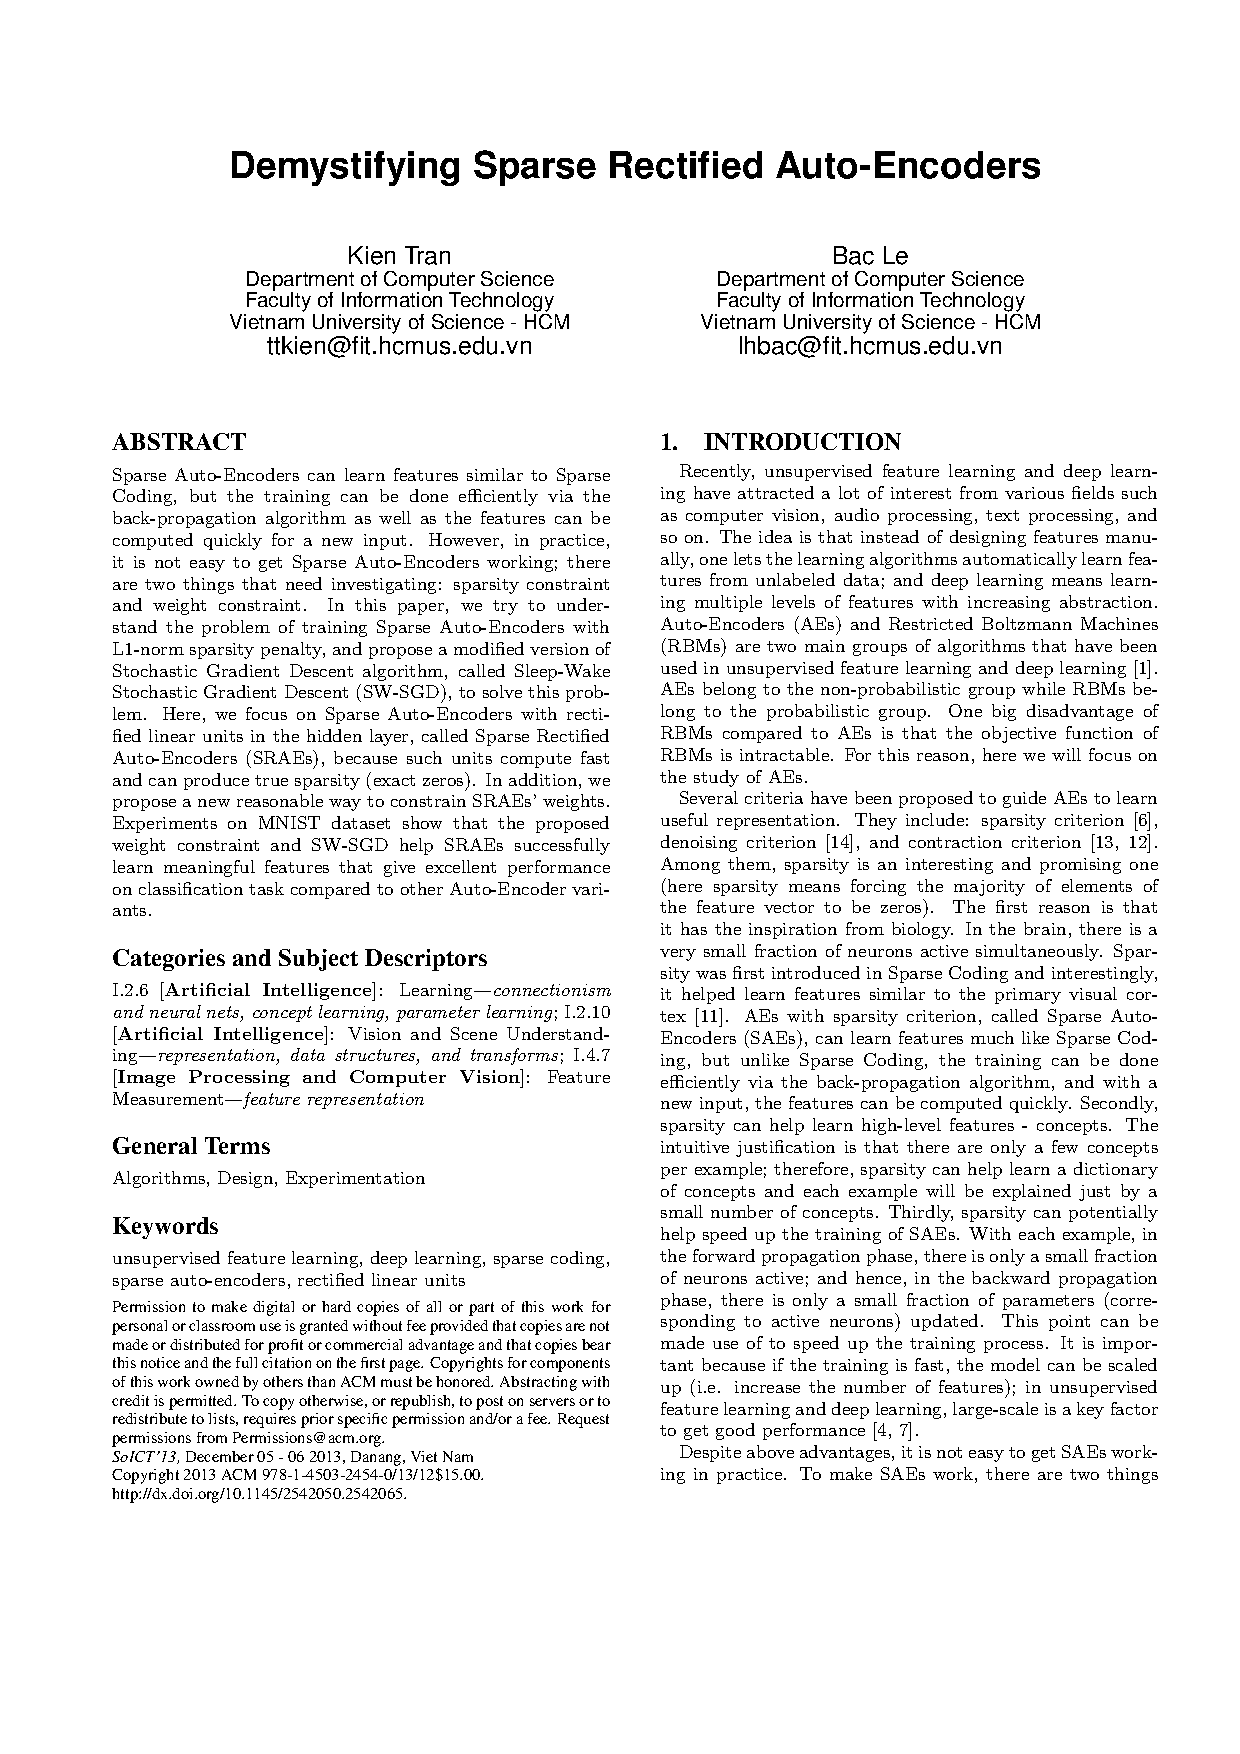
\includepdf[pages=1-7]{docs/MyPaper}

	%\input{Introduction}
	%
	%\input{RelatedWork}
	%
	%\input{Overview}
	%
	%\input{Implementation}
	%
	%\input{Modeling}
	%
	%\input{ExperimentalResults}
	%
	%\input{ApplicationAndFutureWork}
	%
	%\input{Conclusion}
	
	\renewcommand{\bibname}{
		\addcontentsline{toc}{chapter}{TÀI LIỆU THAM KHẢO}
		TÀI LIỆU THAM KHẢO
	}
	\bibliographystyle{Classes/IEEEtranS}
	\bibliographystyle{unsrt}
	\bibliography{References/my_bib}
	
	
	%\input{Appendix}
	
\end{document}